\section{Methodology}
%todo: add introduction to methodology
Many engineering decisions were made during the course of this project. Decisions as large as how any joints the arm would support, and as small as which type would be fitting for a certain variable. These decisions were all made in order to uphold the design goals of our project. 

\subsection{System Design}
%todo: methodology->system design
\begin{figure}[H]
	\centering
	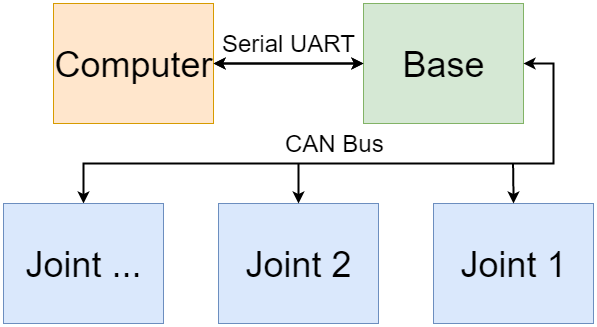
\includegraphics[scale=0.4]{system_coms_diagram}
	\caption{Block diagram of the entire modular arm system}
	\label{fig:system_block_diagram}
\end{figure}


\subsection{Fourth Joint and Existing Arm}
In order to show that our control system can be integrated with other arms, we designed a fourth joint to connect to an existing arm. By showing that we can add a newly designed joint to our existing arm, we are creating a proof-of-concept that shows the versatility of our control system.  The design of the fourth joint was done in Solidworks, a software that allows users to design objects in a 3-D space \cite{Solidworks}. Once we had designed the fourth link, we moved forward to the rapid-prototyping stage where we took our parts designed in Solidworks and converted them to 3-D printable models.  We then used the software Cura \cite{Cura} and the Lulzbot Taz 6 3-D printer \cite{Taz6} to fabricate a first iteration of our fourth joint.  From here we continued to refine our parts and re-print pieces with tighter tolerances until they came together to make a fourth joint that interfaces with our control system. To find drawings of our solidworks parts, please refer to Appendix H \ref{app:SolidworksDrawings}

\subsubsection{Fourth Joint Design}

\begin{figure}[H]
	\centering
	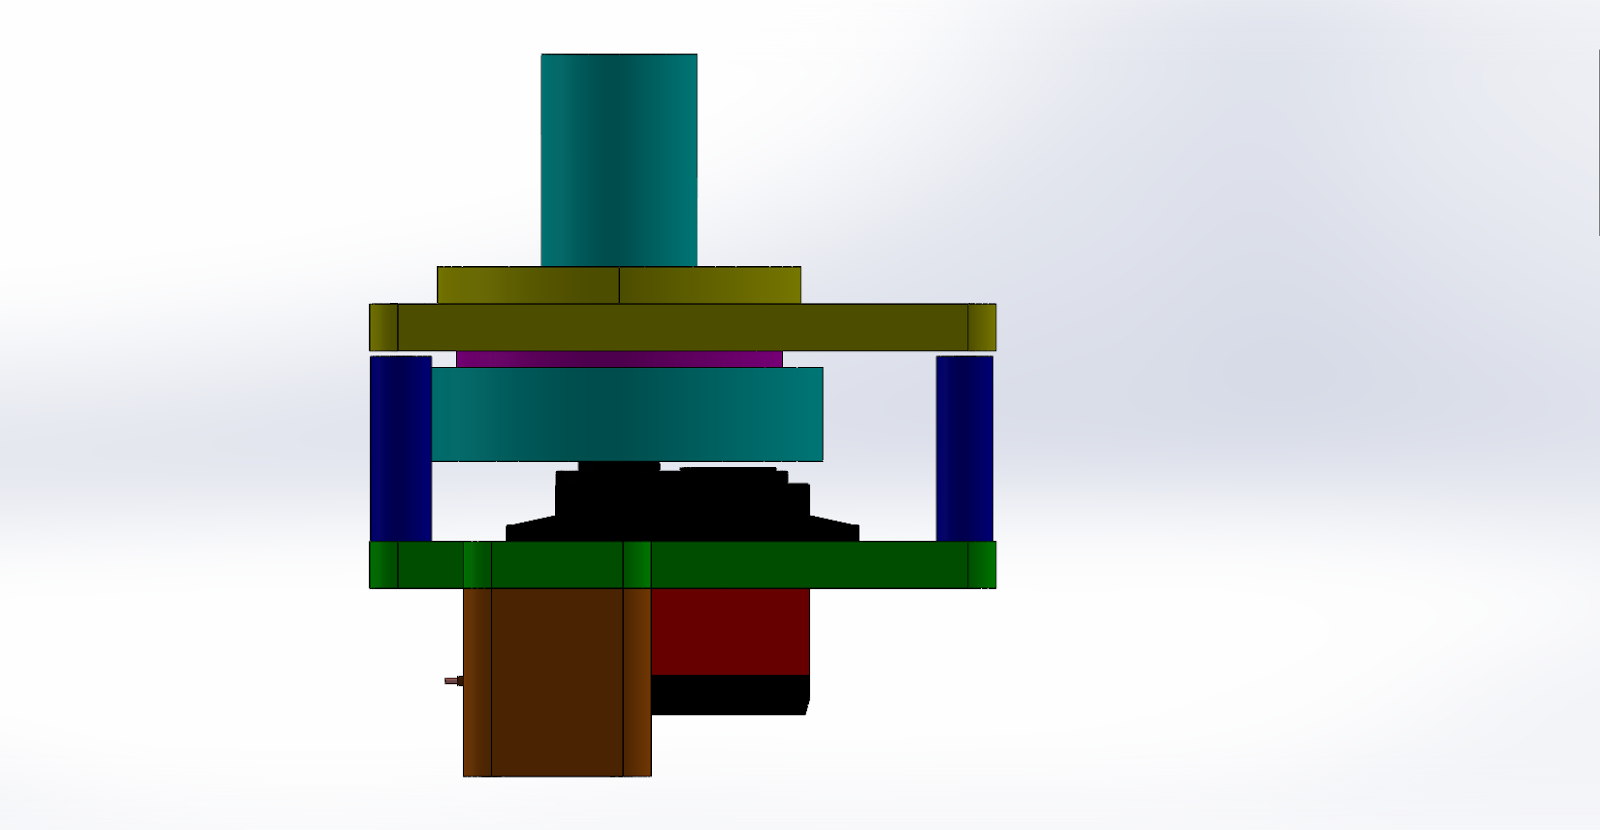
\includegraphics[width=\textwidth/2]{joint4FrontView}
	\caption{Joint 4 CAD Model}
	\label{fig:Joint 4 CAD Model}
\end{figure}

The fourth joint features a shaft which is supported by both a thrust bearing and a radial bearing. It can therefore tolerate loads that are parallel to the shaft, which the arm would encounter when picking objects straight up, as well as loads that are perpendicular to the shaft - forces that generate torques about the base of the motor.\\


\begin{figure}[H]
	\centering
	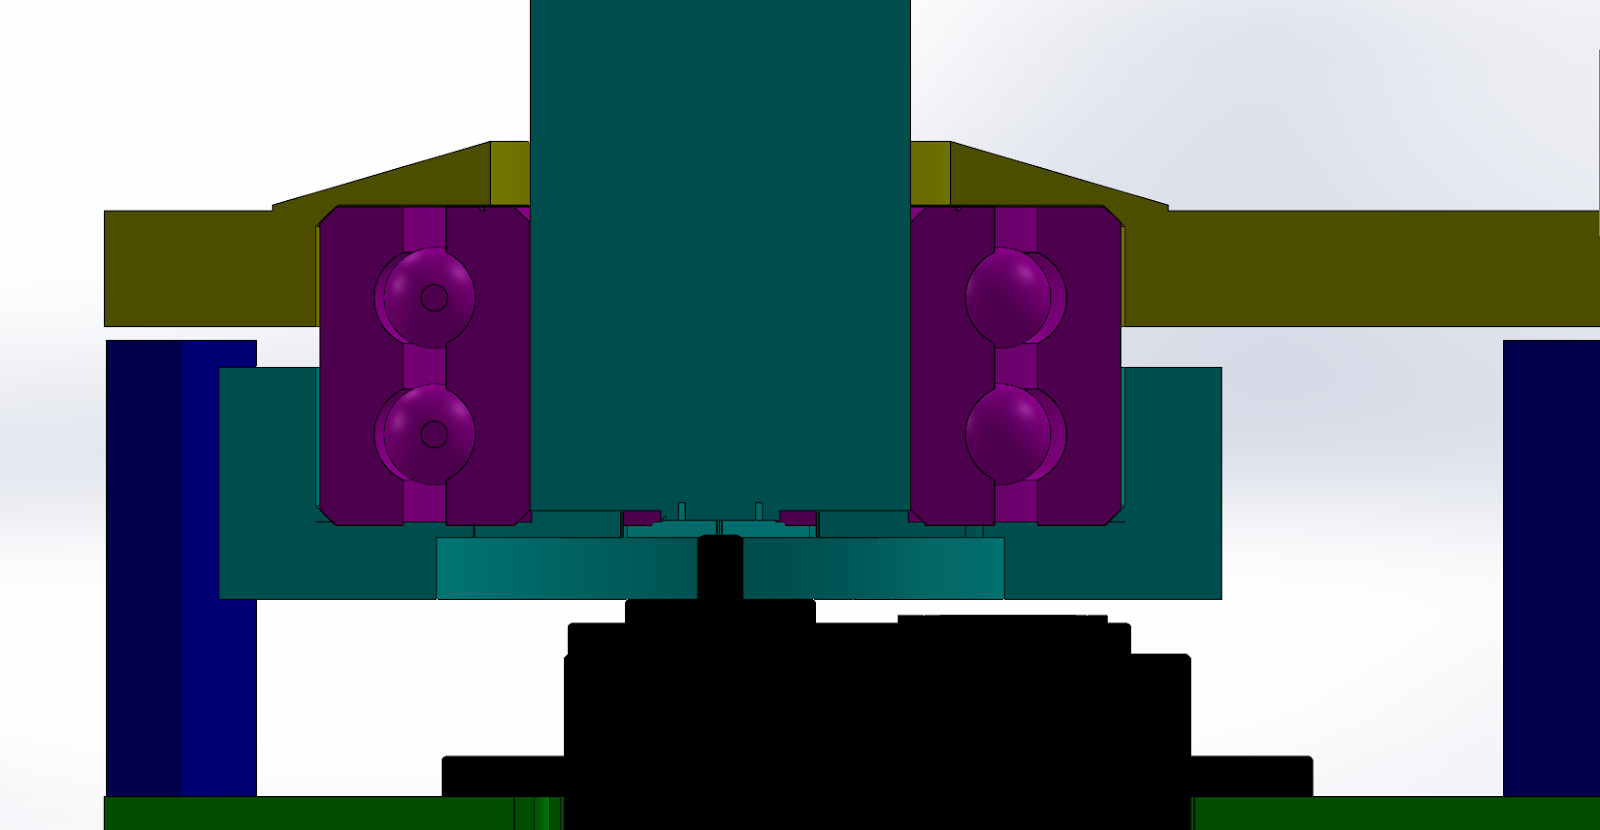
\includegraphics[scale=0.07]{bearingMount}
	\caption{Cutout View of Bearing Mount}
	\label{Cutout View of Bearing Mount}
\end{figure}


\noindent Our decision to create a joint that is actuated using a brushed DC motor was undertaken in order to prove that we can control DC motors in addition to the servos that already exist on the arm.  Next, we decided that since most of the joints currently on the arm provide rotation that results in the end effector moving vertically, we wanted a joint that provides parallel rotation. \\

To accomplish this we removed the control logic from a servo that already was used on the arm, converting it into a brushed DC motor. Next, we designed a direct-drive mount for the motor we fabricated so that the output shaft would rotate along the motor's axis of rotation.  We built a mount for the motor and a structure to provide support for both radial and axial load on the shaft. This structure made use of multiple radial bearings, placed to keep the shaft in line and eliminate any friction between moving and static pieces of the joint.  We also included a thrust bearing on the main shaft in order to stop thrust loads from being placed directly on the servo.  Finally, we designed an idler-shaft that sits in two bearings so that it can freely rotate with negligible friction. The purpose of this idler shaft is to rotate in a 1:1 gear ratio with the main shaft using a timing belt to connect the two shafts.  At the bottom of the idler shaft there is a magnet whose changing magnetic field is read by a Hall effect sensor mounted onto the bottom of the fourth joint so that it sits exactly 1mm from the magnet, allowing for optimal position reading.  \\

\begin{figure}[H]
	\centering
	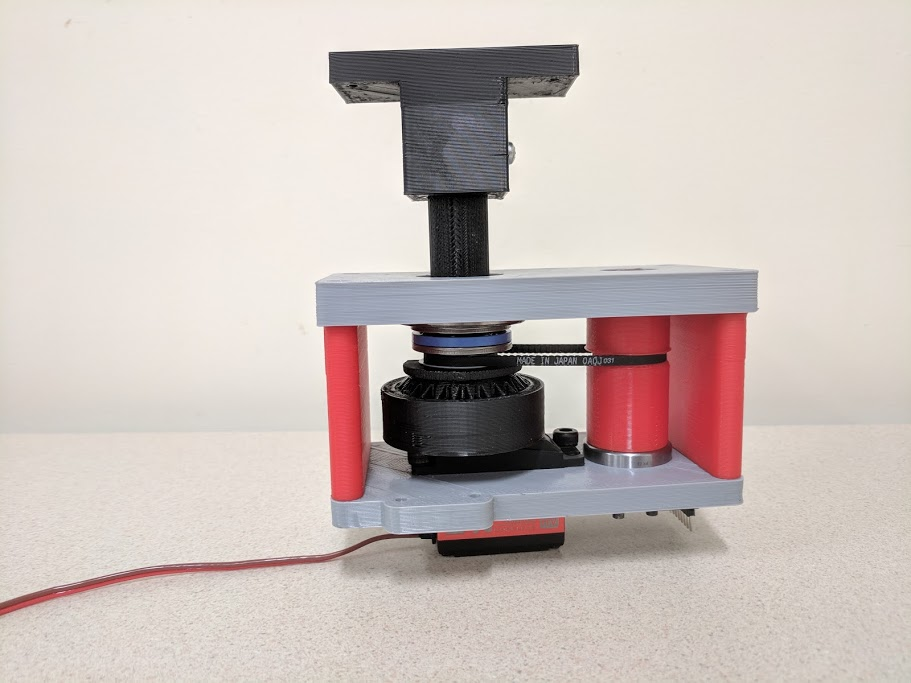
\includegraphics[width=\textwidth/2]{joint_4_with_encoder}
	\caption{Side View of Final Removable Joint}
	\label{fig:Side View of Joint 4}
\end{figure}


\subsubsection{Fourth Joint Prototyping}


The process of prototyping our fourth joint started with creating an interface so that we can connect it to the already existing arm.  We decided for the sake of simplicity and modularity to attach our fourth joint where the current end-of-arm-tooling would normally connect.


\begin{figure}[H]
	\centering
	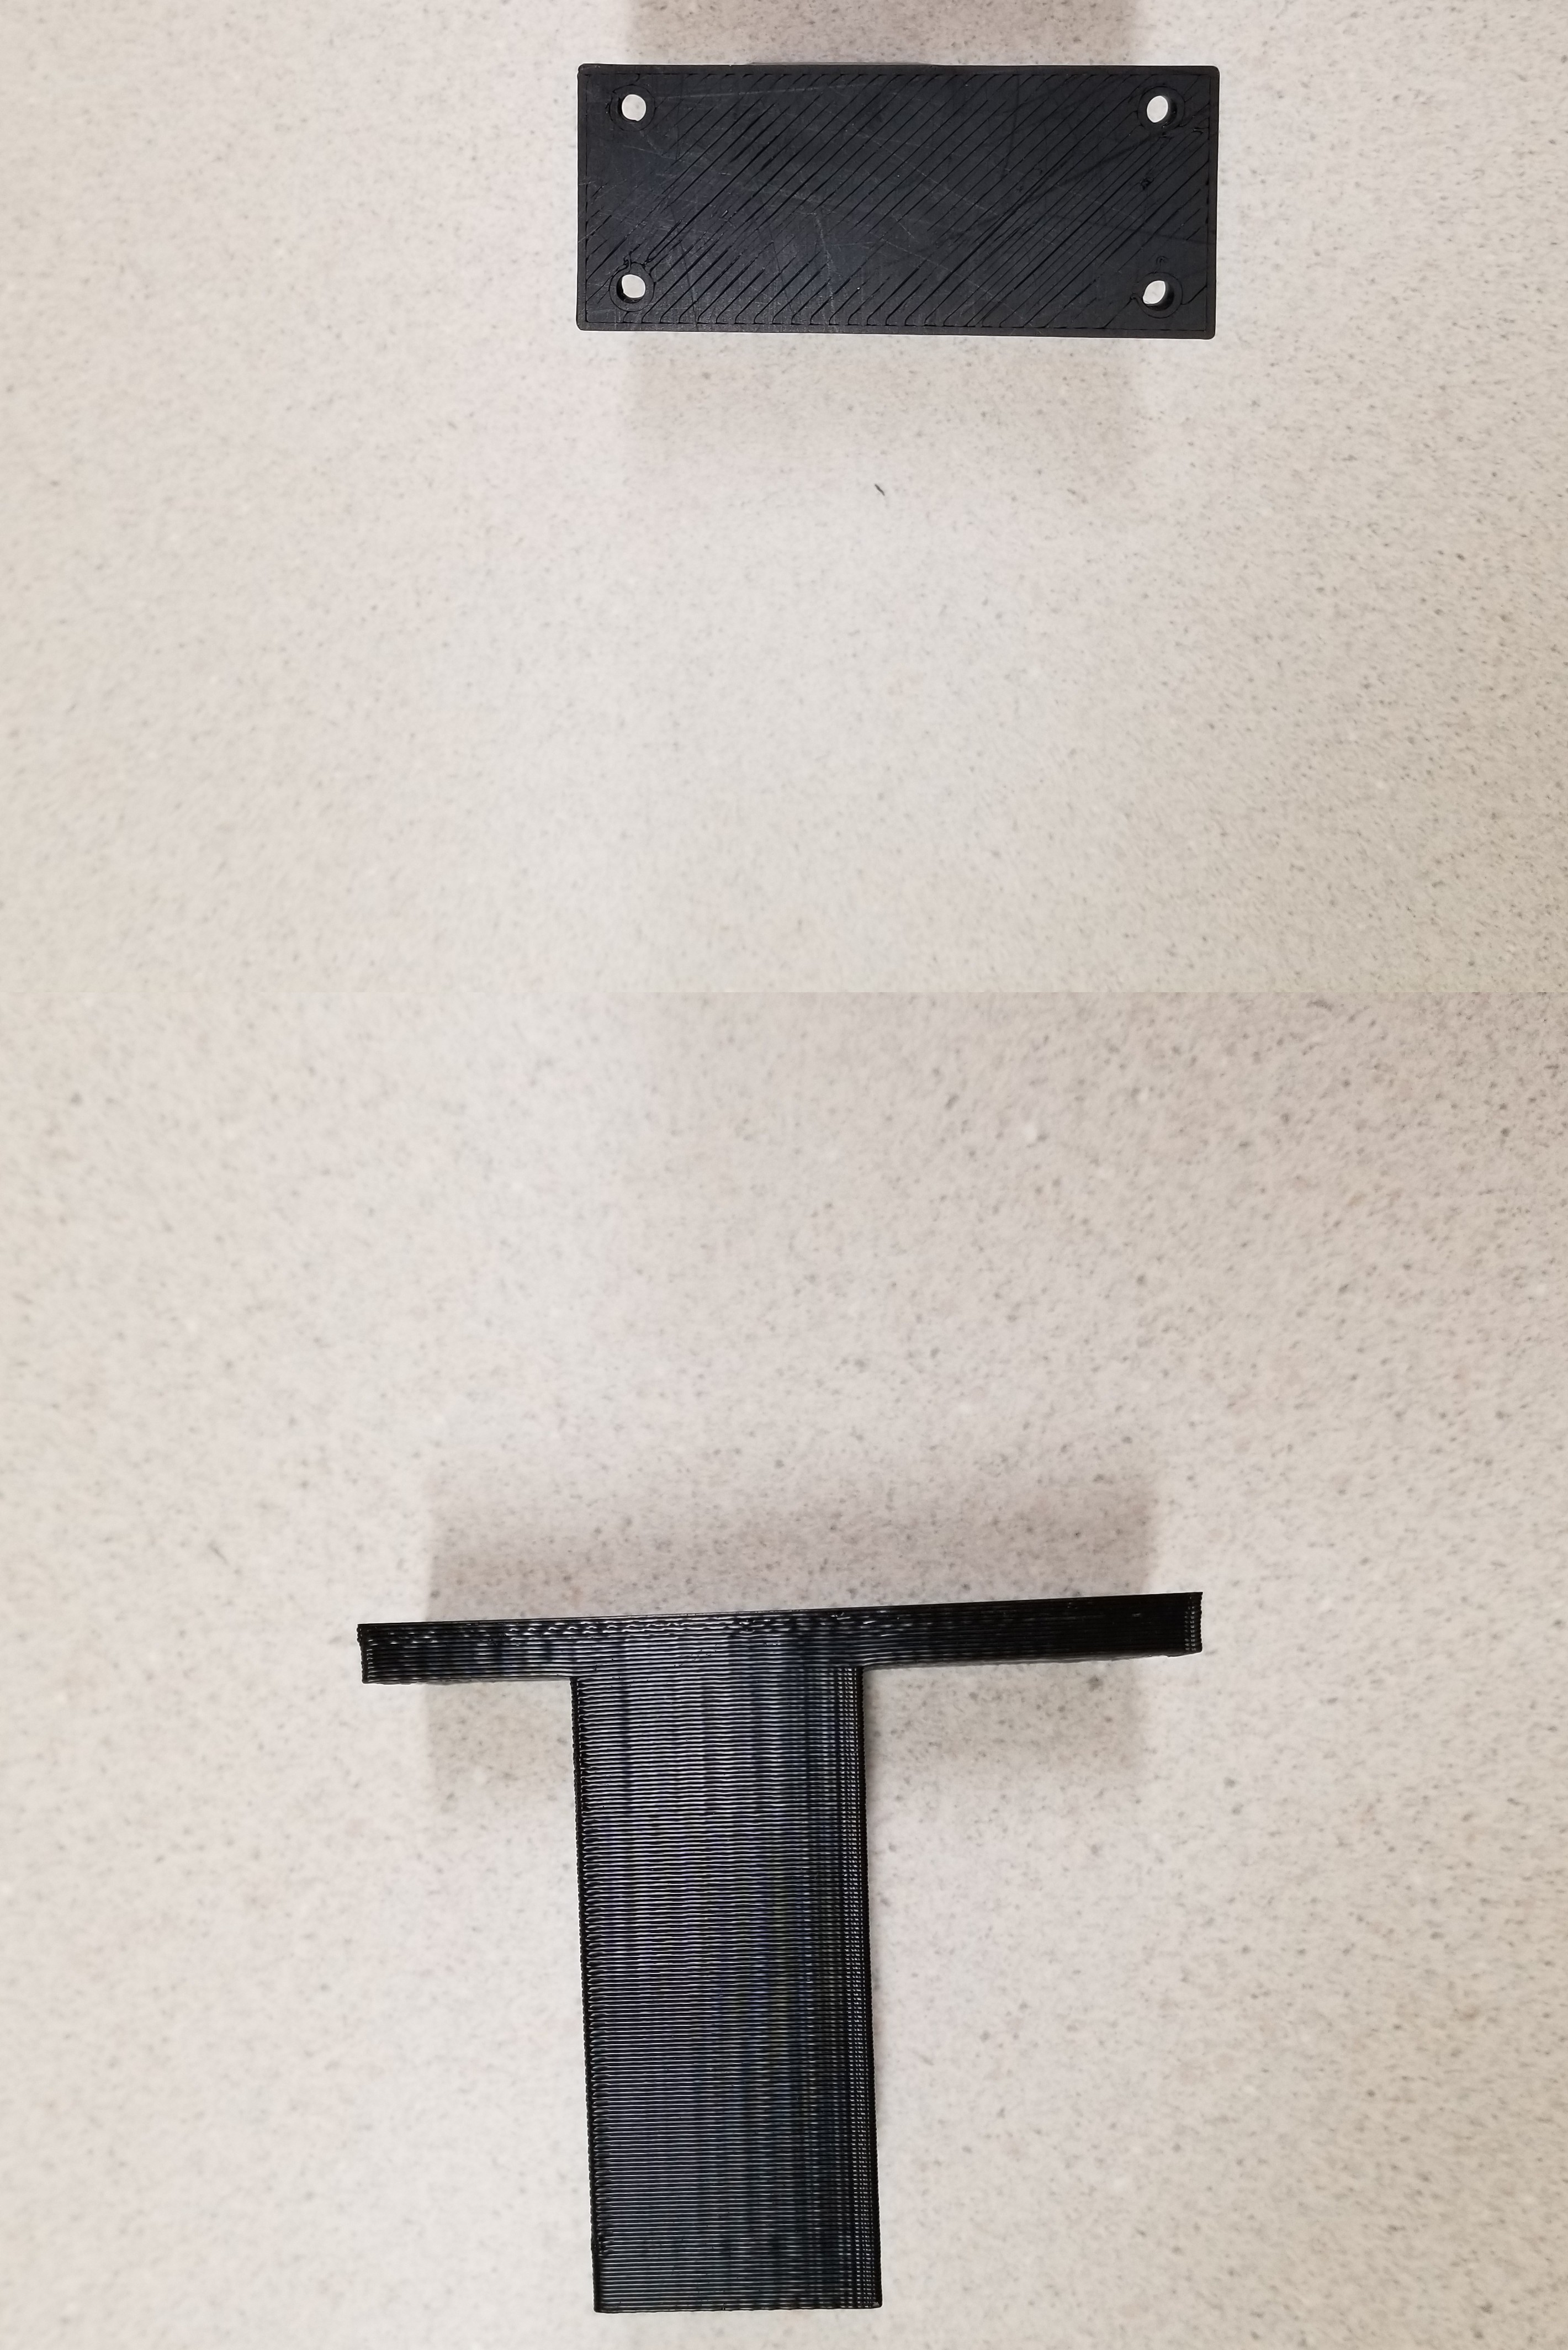
\includegraphics[angle=90, scale=0.07]{current_arm_connector}
	\caption{Current Arm End Effector Mount}
	\label{Current Arm Encoder Mount}
\end{figure}

\begin{figure}[H]
	\centering
	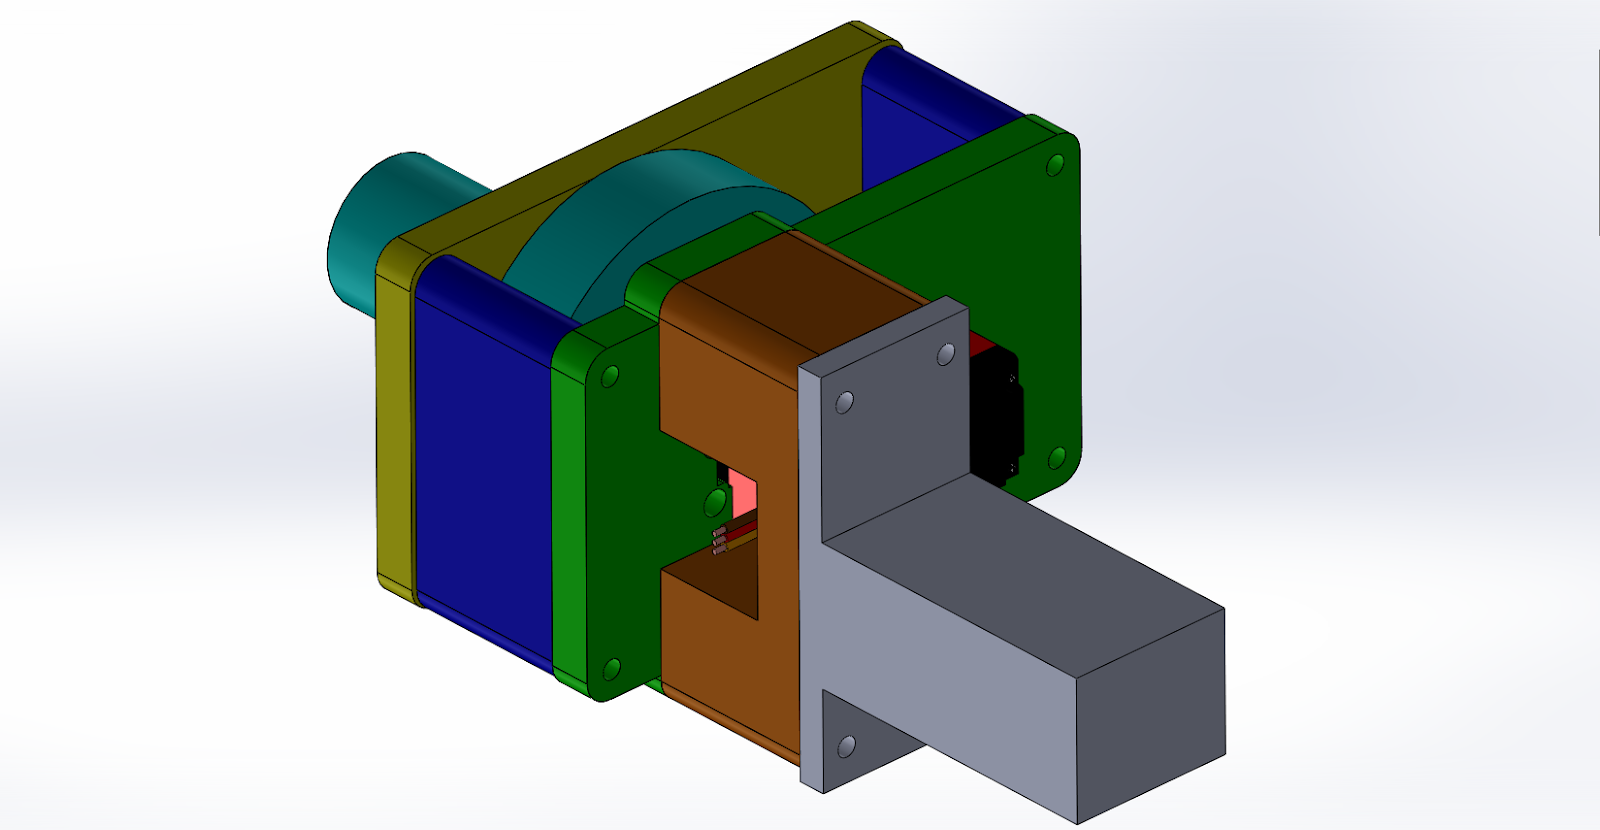
\includegraphics[scale=0.2]{compatibilityWithArm}
	\caption{Joint 4 on End Effector}
	\label{lbl:Joint 4 on End Effector}
\end{figure}

\noindent To create a prototype of our fourth joint, we determined the mechanical requirements of our arm and worked backwards to create a rapid prototyping model (RPM).  RPMs are usually CAD models which are able to be turned into a functional model using a 3-D printer. or other method.  Once the functional model was 3-D printed, we would assemble the parts and test how they all fit together.  With each new functional model we revised our RPM and printed a new functional model in order to meet the requirements for our fourth joint. This process of building, revising based on testing a physical prototype was only made possible due to the advances in recent years in 3-D printing technology making it feasible to create these prototypes so quickly while still having them be robust. 


\subsubsection{3-D Printing}
3-D printing is convenient because it allows the user to manufacture parts in a novel way. Overall, we chose to 3-D print our fourth joint because it was what we were most familiar with and we had easy access to multiple 3-D printers.  While the process of 3-D printing a part might not be as accurate as other more conventional methods of machining parts, it is a much easier method to learn and has a much quicker turnaround time. For our choice of 3-D printer, we used the LulzBot Taz 6 \cite{Taz6} with a single extruder head (Version 2.1) and 2.65mm filament. This printer is readily available to us through the Undergraduate Robotics Lab. The resolution of the printer was fine enough that it was easily able to achieve the tight tolerances needed to print parts such as the timing belt teeth.  

\begin{figure}[H]
	\centering
	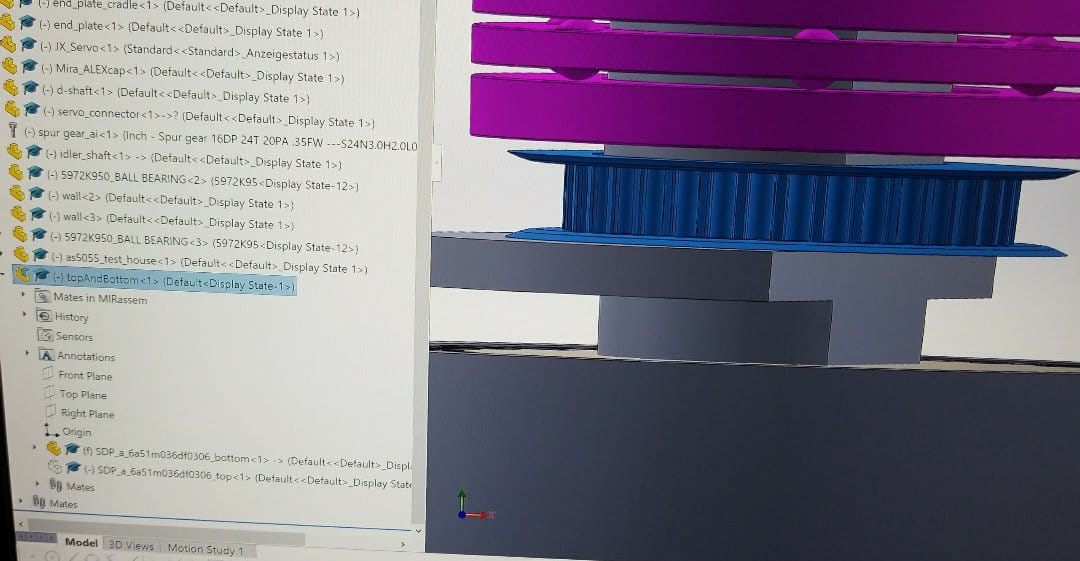
\includegraphics[scale=0.3]{cadPulley}
	\caption{CAD Model of 3D-printable Pulley}
	\label{CAD Model of 3D-printable Pulley}
\end{figure}

%TODO: Those pretty calculations from Chris's notebook that show that the small part won't be crushed

\subsubsection{Motor Selection}

The performance of a DC motor can be characterized by measuring several key values: the stall torque, the stall current, the free running RPM, and the free running current. It's important that all the values be measured when the motor is given the same input voltage.\\

\noindent
Specifications:\\
\noindent
\indent Voltage: 8.4V \\
\indent Stall torque: 32.3 kg cm stall \\
\indent Stall current: 5.25 A stall \\
\indent Free running RPM: 0.1 seconds/60 degrees (100 rpm) \\
\indent Free running current: 0.23 A \\





\begin{table} [H]
	\centering
	\caption{HV5923MG Motor Curve Data from experimental testing}
	\label{tab:MotorData}
	\begin{tabular}{|p{1cm}|p{1.2cm}|p{1.4cm}|p{1cm}|p{1cm}|p{1.5cm}|p{1cm}|p{1cm}|p{1.1cm}|}
		\hline
		Speed (RPM) & Torque (N-m) & Torque (in-lbf) & Current (A) & $P_{out}$ (W) & Efficiency (\%) & $P_{in}$ (W) & Heat (W) & back-EMF (V) \\
		\hline
		
		0 & 3.16 & 27.98 & 5.25 & 0 & 0 & 44.1 & 44.1 & 0 \\
		
		7 & 2.94 & 26.02 & 4.9 & 2.15 & 5.24 & 41.15 & 38.99 & 0.56 \\
		
		13 & 2.75 & 24.34 & 4.6 & 3.74 & 9.69 & 38.62 & 34.87 & 1.04 \\
		
		20 & 2.53 & 22.38 & 4.25 & 5.3 & 14.85 & 35.67 & 30.37 & 1.61 \\
		
		27 & 2.31 & 20.42 & 3.89 & 6.52 & 19.94 & 32.71 & 26.19 & 2.17 \\
		
		33 & 2.12 & 18.74 & 3.59 & 7.32 & 24.24 & 30.18 & 22.87 & 2.65 \\
		
		40 & 1.9 & 16.79 & 3.24 & 7.94 & 29.17 & 27.23 & 19.29 & 3.21 \\
		
		47 & 1.68 & 14.83 & 2.89 & 8.24 & 33.96 & 24.28 & 16.04 & 3.78 \\
		
		53 & 1.49 & 13.15 & 2.59 & 8.24 & 37.9 & 21.75 & 13.51 & 4.26 \\
		
		60 & 1.26 & 11.19 & 2.24 & 7.94 & 42.25 & 18.8 & 10.86 & 4.82 \\
		
		67 & 1.04 & 9.23 & 1.89 & 7.32 & 46.18 & 15.85 & 8.53 & 5.38 \\
		
		73 & 0.85 & 7.55 & 1.59 & 6.52 & 48.99 & 13.32 & 6.79 & 5.86 \\
		
		80 & 0.63 & 5.6 & 1.23 & 5.3 & 51.09 & 10.37 & 5.07 & 6.43 \\
		
		87 & 0.41 & 3.64 & 0.88 & 3.74 & 50.49 & 7.41 & 3.67 & 6.99 \\
		
		93 & 0.22 & 1.96 & 0.58 & 2.15 & 44.12 & 4.88 & 2.73 & 7.47 \\
		
		100 & 0 & 0 & 0.23 & 0 & 0 & 1.93 & 1.93 & 8.03 \\
		\hline
		
	\end{tabular}
	
\end{table}

\begin{figure}[H]
	\centering
	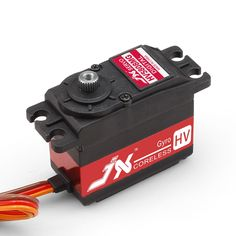
\includegraphics{motor}
	\caption{HV5923MG Servo Motor}
	\label{fig:HV5923MG Servo Motor}
\end{figure}


\subsubsection{Arm Base}
% Talk about requirements for base
% take in new joint data at certain speeds
% output new joint data at certain speeds
The mechanical side of the base module is relatively simple because the physical structure comes from the pre-existing arm. In order to make this compatible with our controls system, all we have to do is mount our joint and encoder boards to it. This is fairly simple since we use a slightly modified version of the encoder board on the existing arm with the same mounting scheme. Our joint board mounting scheme focused around mounting each board in a place where it would not be impeded by the movement of the arm during runtime. 

\begin{figure}[H]
	\centering
	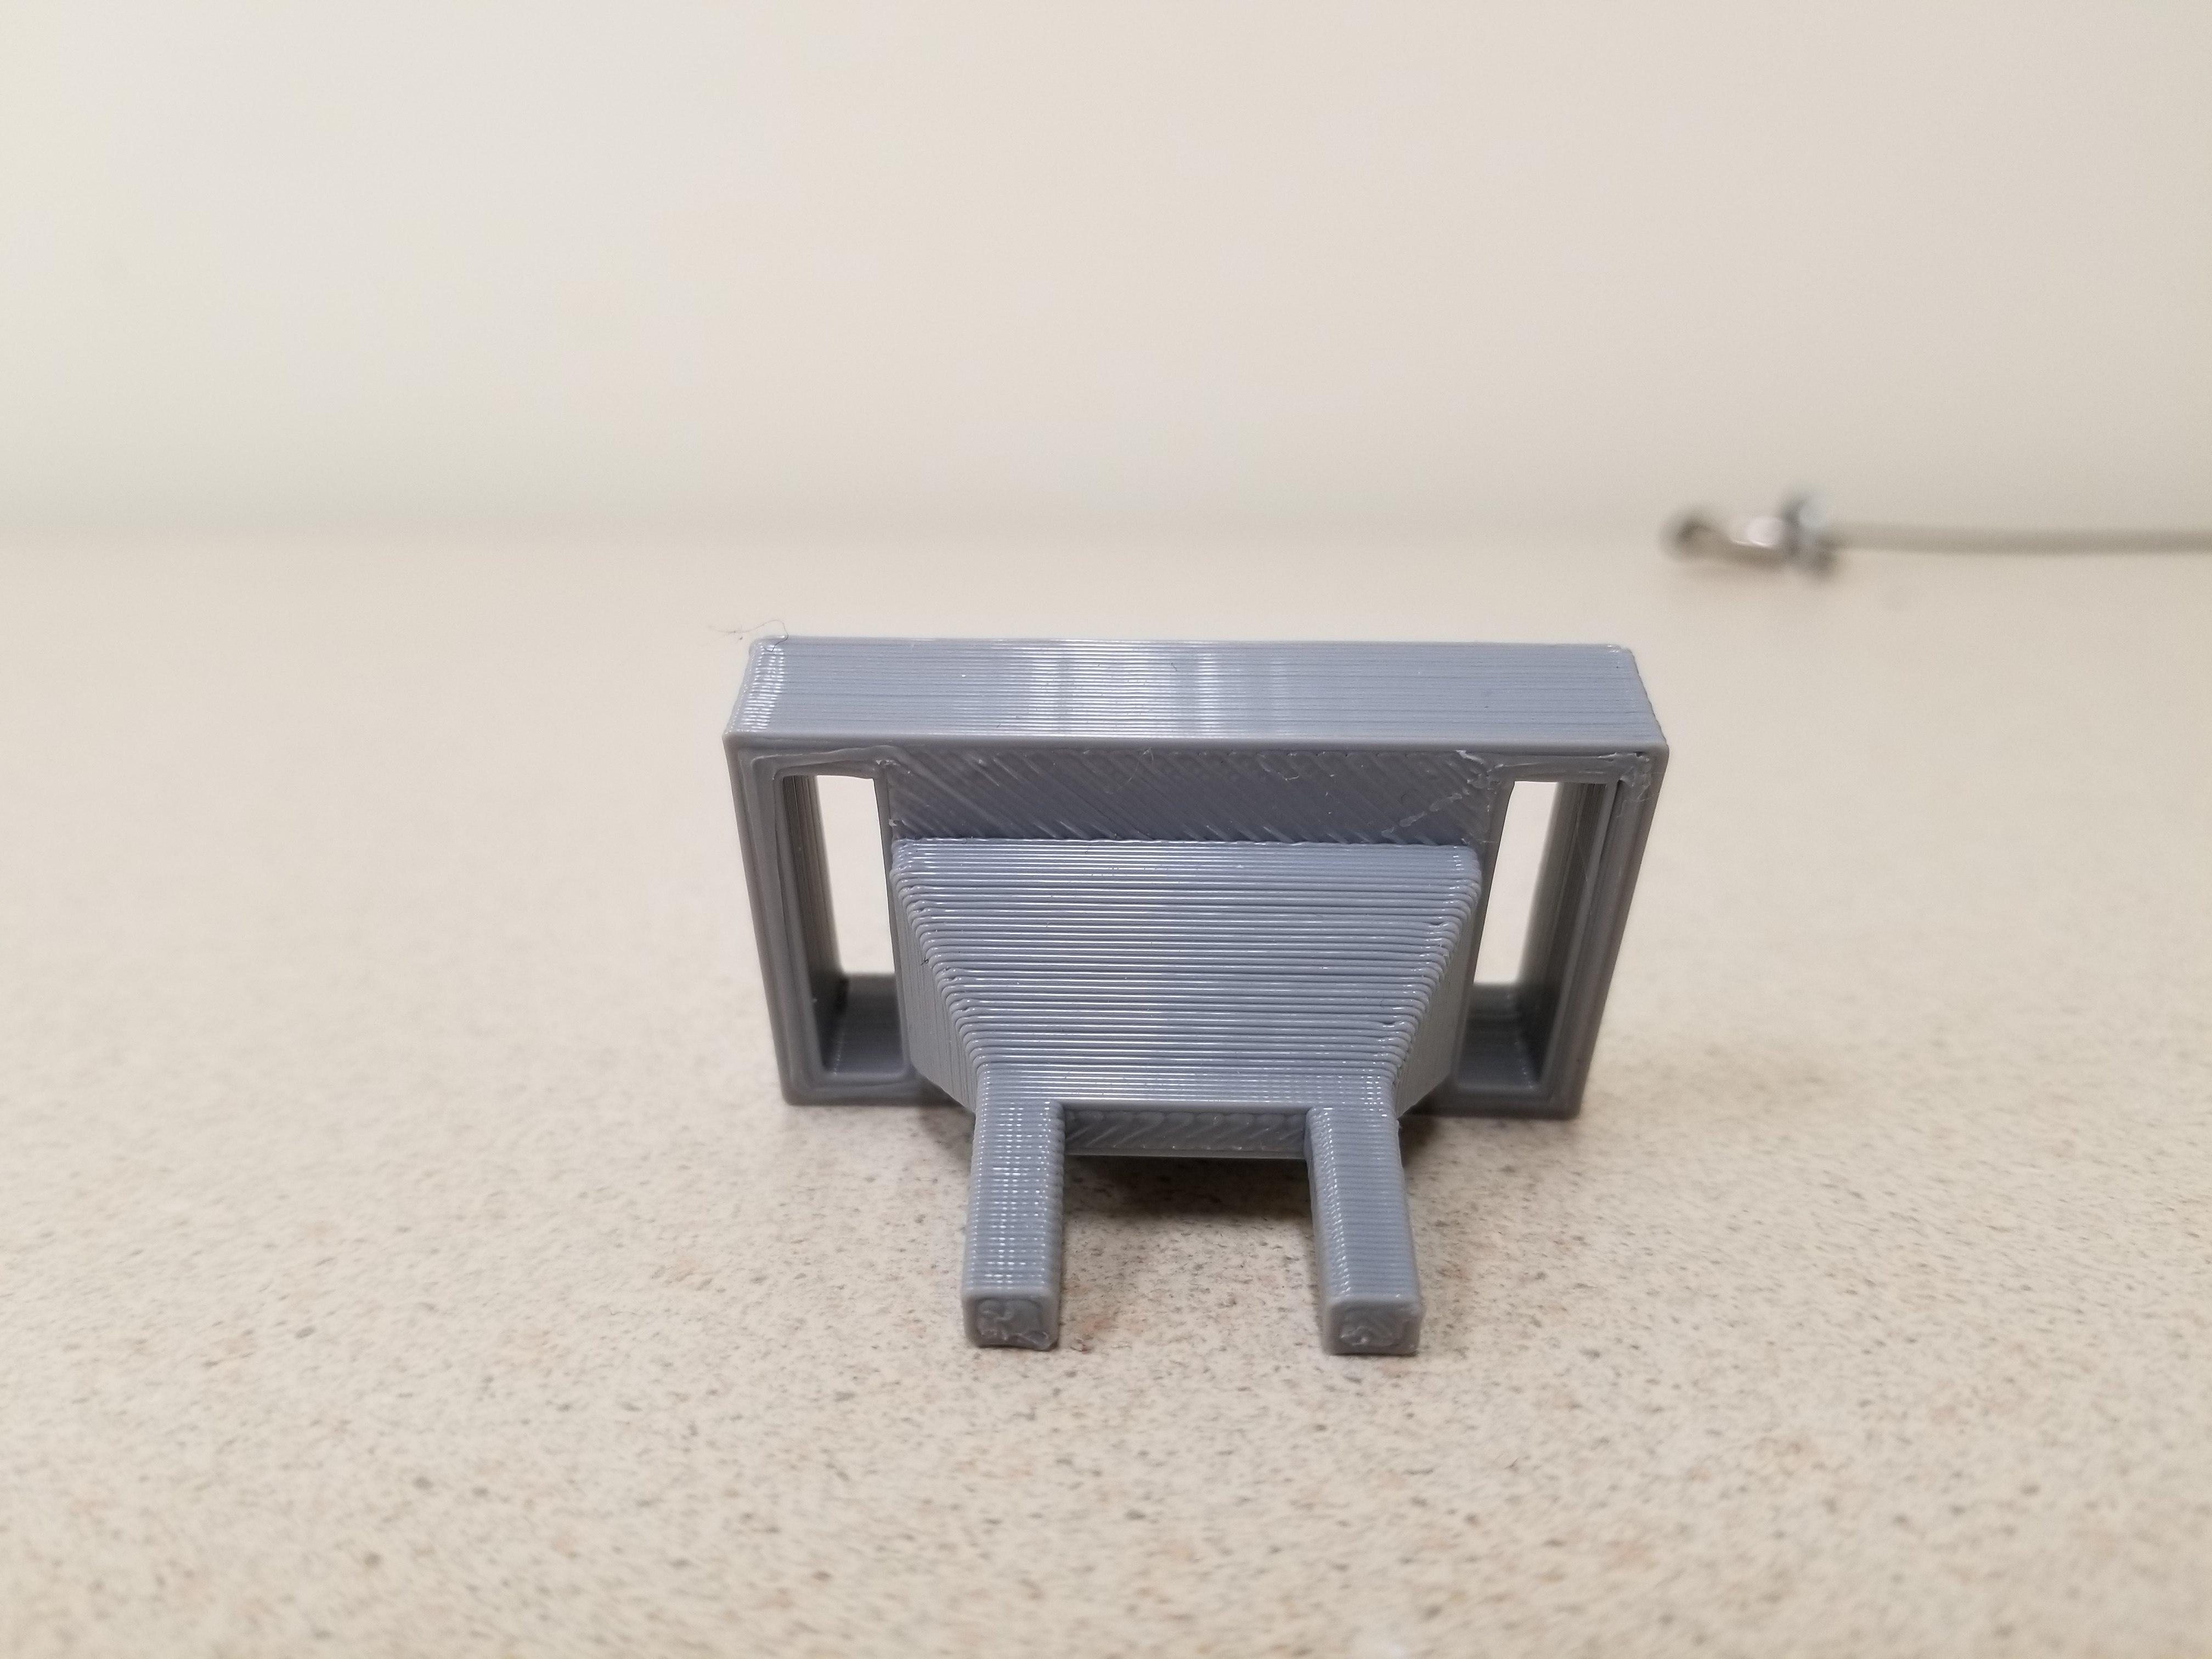
\includegraphics[width=\textwidth]{mount_back_view}
	\caption{TM4C123G to arm mount}
	\label{fig:mount_back_view}
\end{figure}

\begin{figure}[H]
	\centering
	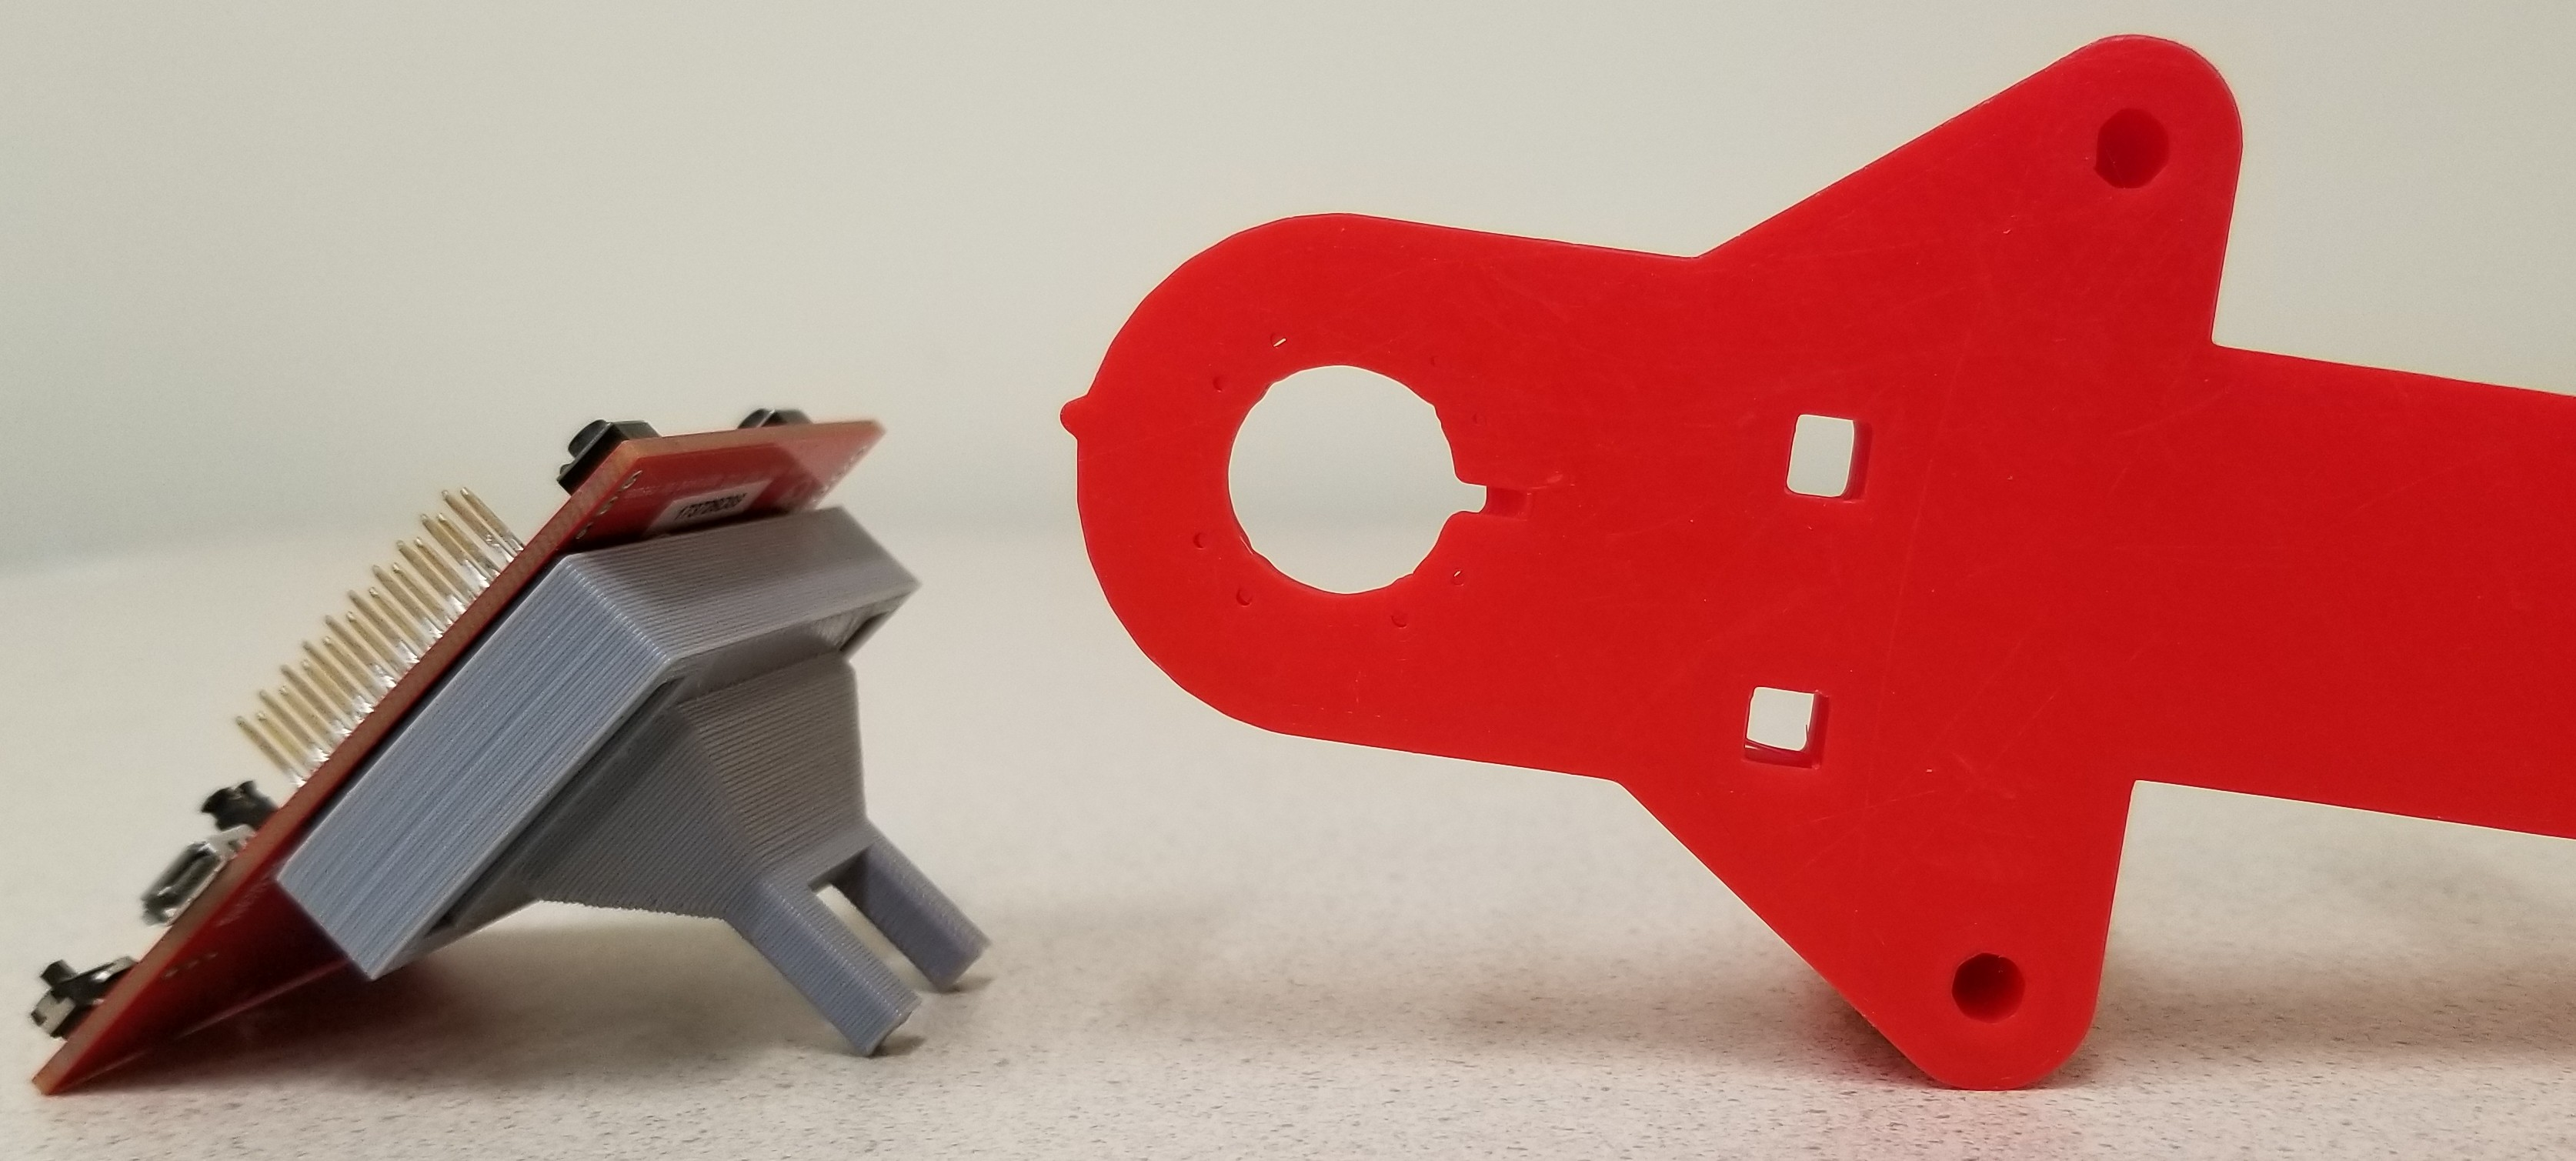
\includegraphics[width=\textwidth]{mount_and_holes}
	\caption{Mounting holes on arm and mounted TM4C123G}
	\label{fig:mount_and_holes}
\end{figure}

\noindent We have not only made sure that none of the mechanical components of the arm would come into contact with the board but also that none of the wiring between boards would be unplugged. This meant that we had to mount the boards far enough away from moving parts while still keeping it close enough to the sensors and motors that needed to interface with it. We decided to mount it in the same position for each category of joint type to keeps these needs consistent. Making use of an already existing area used to mount the cabling for the previous iteration of the arm seemed like the most efficient way to go about this. We designed a mechanical interface that was able to press-fit into our joint board and connect to the previous mounting solution.


\subsection{Joint Control Board}
The joint control board sits at the heart of the entire functionality of the project. Without a robust and capable design, any arm constructed would not function properly. Selecting the types of sensors to use for the control board was a very important step of the joint control board design. %todo FINISH THISS

\subsubsection{Overview of Design}
The joint board underwent significant revisions, outlined in Section \ref{sec:pjcbd}, but the depth of revision significantly dropped after the decision was made to use the TM4C123GH6PM 32-bit ARM processor. This processor had many peripherals internally that simplified the joint board design significantly. A block diagram of the final joint control board can be seen in Figure \ref{fig:jcb_block_diagram}.

\begin{figure}[H]
	\centering
	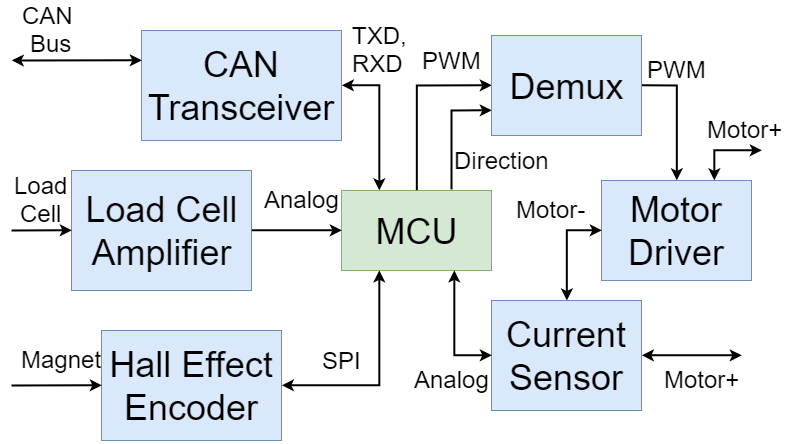
\includegraphics[scale=0.4]{jcb_block_diagram}
	\caption{Block diagram of the joint control board}
	\label{fig:jcb_block_diagram}
\end{figure}

\subsubsection{Joint Angle Sensor}
\label{sec:jas}
As mentioned in Section \ref{sec:control_board}, joint angle sensing is one of the main tasks needed in order to control a robot arm. Without this key sensor, the robot arm controller has no way of knowing where its links actually are in space. The type of sensor is very important since each has different design considerations that need to be taken into account.

\noindent Potentiometers seem like a good choice due to their simplicity and high accuracy capabilities. However, they do not lend themselves well to this application because of how quickly they wear out. Over time, as the joints move to different positions, the potentiometers will wear out quickly and cause inaccurate readings. Additionally, long lifespan and high resolution potentiometers can be very expensive. Furthermore, potentiometers are large and can be difficult to mount. Finally, the hard stop on the potentiometer means the joint angles will be limited to a certain range (typically about 270 \textdegree for single turn potentiometers).

\noindent The next obvious solution is to use optical encoders because they will not wear out and offer very high resolution capabilities. These sensors are not well suited for this application, however, since they are typically expensive, especially for high resolution encoders - and ones that are capable of reading absolute position. Additionally these sensors are somewhat bulky and would take up too much space in the closed environment of a joint. 

\noindent This leaves us with Hall effect sensors. These sensors are very small and moderately high resolution while also being a contact-free sensor, so wearing them out will not be a concern. A main concern with Hall effect sensors is that they need to be mounted somewhat precisely and carefully. Traditional machining methods make this difficult to accomplish, but 3D printing allows us to easily overcome this challenge.  Another concern is external electromagnetic interference, but with somewhat careful circuit board design, we should be able to minimize this issue.

\subsubsection{Motor Current Sensor}
As mentioned in Section \ref{sec:control_board}, the motor current is another important factor in controlling a robot arm. Since motor current is proportional to motor torque, knowing the current lets the controller know how much force the arm is putting on a load, to give an example. There are a few different technologies that can sense the current through a motor, each with their own design considerations that must be taken into account.

\noindent A shunt resistor seems practical due to the simplicity of the design, but careful tuning must be done in order to get the noise levels down to a reasonable amount. In addition to this, the power loss when using a shunt resistor could cause the arm to stall before anticipated. When the shunt resistor takes power from the motor, the whole motor curve slides inward, decreasing the maximum power output. Trace resistance would be a good alternative, but requires calibration after the circuit is constructed. 

\noindent Instead of these, we decided to use a Hall effect current sensor. Hall effect current sensors are ready-made sensors that give low noise, properly calibrated outputs, are not very expensive, and are easy to integrate into a circuit design. These sensors have extremely small power losses to the motor. The main drawback of these sensors is that they have a low bandwidth, but we are using DC motors so this should not be a problem. Some care will need to be taken when placing these on the circuit, however, since they are sensitive to external magnetic fields. The hall effect current sensor chosen for this design was the ACS722. This device was selected by using Table \ref{tbl:Current Sense IC Comparison}.

\begin{table}[H]
	\centering
	\caption{Current Sense IC Comparison}
	\begin{tabular}{|p{4.2cm}|p{1.5cm}|p{2cm}|p{1.7cm}|c|p{1.4cm}|}
\hline
Part name & Supply Voltage (V) & Current Range (A) & Sensitivity (mV/A) & Output & Built in filter? \\
\hline

ACS722LLCTR-05AB & 3.3 & -5 to +5 & 264 & Analog & y \\

ACS723LLCTR-05AB & 5 & -5 to +5 & 400 & Analog & y \\

ACS724LLCTR-10AB & 5 & -10 to +10 & 200 & Analog & n \\

ACS725LLCTR-10AU & 3.3 & 0 to +10 & 264 & Analog & n \\
\hline

\end{tabular}

	\label{tbl:Current Sense IC Comparison}
\end{table}

\subsubsection{Inter-board Communication}
Inter-board communication is the heart of any arm. Without this, the joints of an arm wouldn't know where how to move. A good, robust communication protocol that allows for simple transactions between boards is favorable for this application.

\noindent SPI and I$^2$C are mostly used for on-board, controller-to-peripheral communications and therefore are not a good choice for the base to control board communication. RS232 is not a good solution for this problem either because it is a single transmitter and single receiver per line. This leaves RS485 and CAN.

\noindent RS485 and CAN are similar in many ways, but with a few key differences that separate them. RS485 is very fast to transmit and simple to implement, but takes a lot of the controller's time to send packets. CAN has the advantage because the controller and transceiver control the transmission independent of the controller so the controller has more free time to process data. Another advantage CAN has over RS485 is the amount of error checking that goes on to ensure proper message transmission. For these reasons, we decided to use CAN to communicate between the base and control boards.

\subsubsection{Preliminary Joint Control Board Designs}
\label{sec:pjcbd}
Preliminary joint control board design was done very early on in the project. Unfortunately, the majority of this work was done before much of the necessary research for part selection, leading to many revisions and re-designs, though the main concepts stayed in place. This section outlines the preliminary designs and revisions of those up until the selection of the TM4C123GH6PM microcontroller, at which point the design solidified and forward progress began. 

\begin{figure}[H]
	\centering
	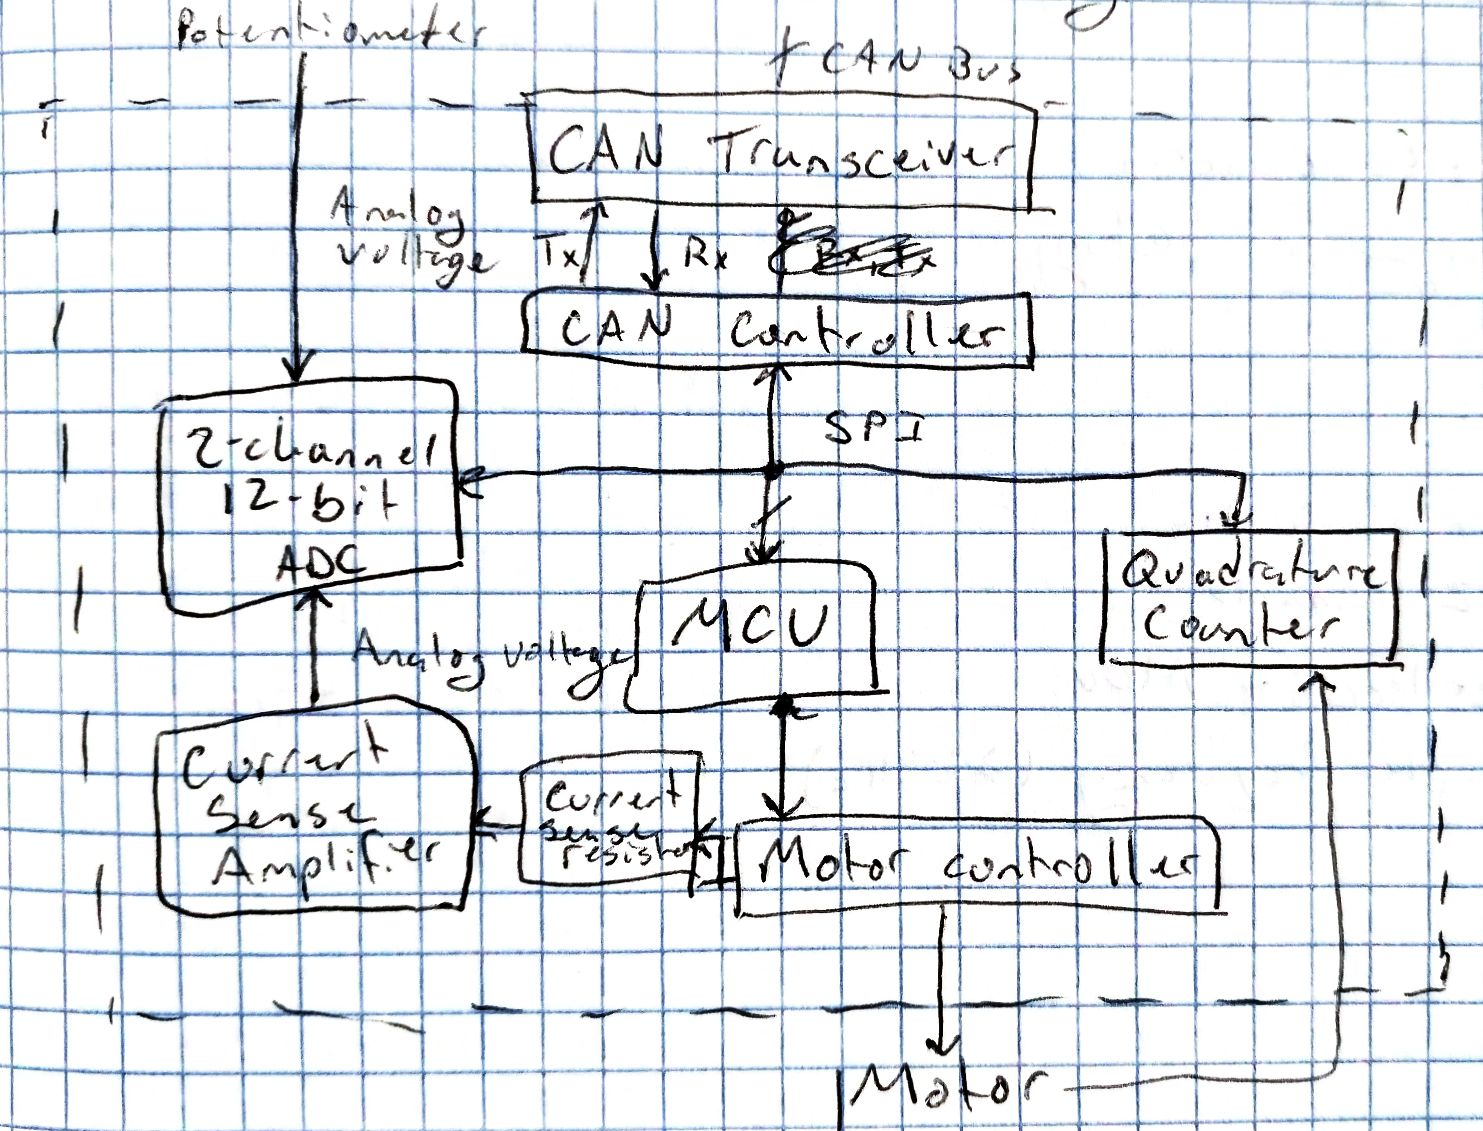
\includegraphics[scale=0.18]{first_joint_board_block_diagram}
	\caption{First draft of the complete joint board block diagram}
	\label{fig:1st_joint_board_block}
\end{figure}

\noindent The first complete block diagram of the joint control board Figure \ref{fig:1st_joint_board_block}. This diagram was centered around a MSP430G series microcontroller, and focused on keeping the cost of the board down. Some component selection was solidified , including the following: MSP430G2553 (microcontroller), MCP3202 (ADC), DRV8872 (motor driver), LS7366R (quadrature counter), MCP2515 (CAN controller), and MCP2561 (CAN transceiver). 

\noindent The decision to replace the potentiometer with an absolute hall effect encoder was made to lengthen the lifespan of the device. Greater detail about this decision is presented in Section \ref{sec:jas}. This change resulted in the diagram shown in Figure \ref{fig:nice_prelim_joint_board_block}. Certain components, such as the CAN controller and transceiver, operated at 5V while others, such as the microcontroller and absolute hall effect encoder, required 3.3V. Most other components could function at either voltage, and were placed on either side of the level shifter for other reasons. The ADC, for example had a supply-voltage-dependent maximum SCLK frequency.
\begin{figure}[H]
	\centering
	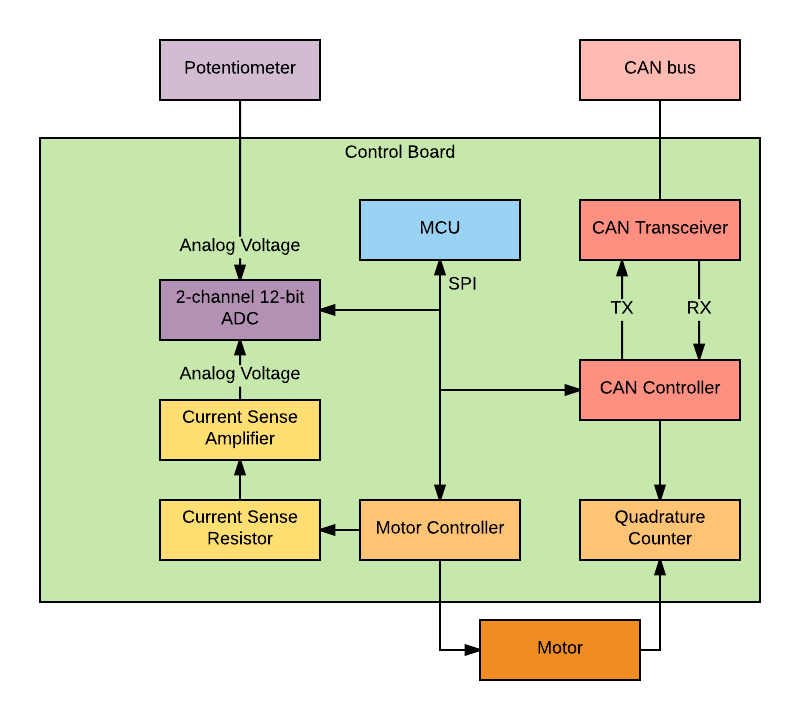
\includegraphics[scale=0.3]{link_block_diagram}
	\caption{Iteration of preliminary joint board block diagram}
	\label{fig:nice_prelim_joint_board_block}
\end{figure}

\noindent Some planning was done to coordinate communication between the components, including placement of a 3.3V to 5V level shifter. This planning led to the block diagram shown in Figure \ref{fig:2nd_joint_board_block}. This diagram requires many lines to pass through the level shifter, which is not ideal and led to the decision to revise component selection.

\begin{figure}[H]
	\centering
	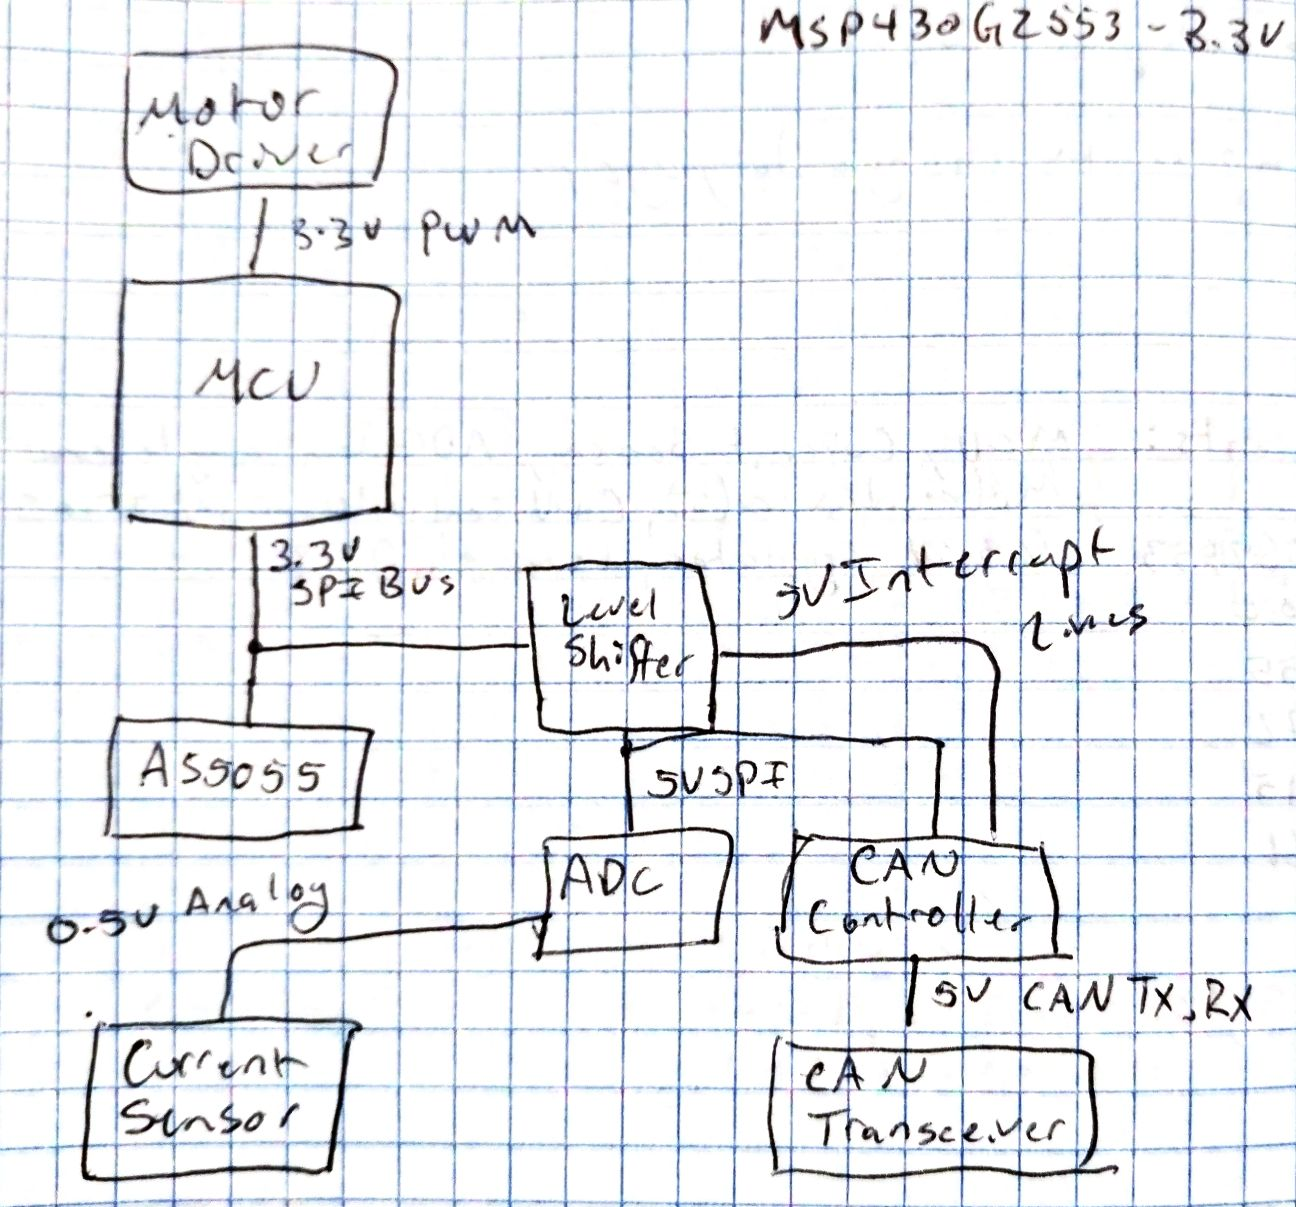
\includegraphics[scale=0.2]{second_joint_board_block_diagram}
	\caption{Mostly complete preliminary joint board block diagram}
	\label{fig:2nd_joint_board_block}
\end{figure}

\subsubsection{ADC Selection}
The first design of the joint control board used a potentiometer to detect the joint angle and a current sense amplifier to detect the motor current. Both of these signals require an ADC to process, and the original microcontroller did not have a high resolution ADC on board, so an off board ADC was needed. Table \ref{tbl:ADC Selection} highlights the different ADCs that were evaluated before selecting one. The MCP3202, while not necessarily the best option from the chart, was selected since it has a very easy to use interface and was available in DIP package for easy testing. With the switch from the MSP430G2553 to the TM4C123GH6PM, the external ADC was no longer needed.

\begin{table}[H]
	\centering
	\caption{ADC Selection}
	
	\begin{tabular}{|c|c|c|c|c|}
		\hline
		& Supply & Sampling & SCLK & \\
		Part name & Voltage (V) & rate (MHz) & Freq (MHz) & Price (\$) \\
		\hline
		ADS7042 & 3.3 & 1 & 16 & 2.65 \\
		
		ADS7043 & 3.3 & 1 & 16 & 2.65 \\
		
		ADS7044 & 3.3 & 1 & 16 & 2.65 \\
		
		ADC121S021 & 3.3, 5 & 0.2 & 4 & 2.85 \\
		
		ADC121S051 & 3.3, 5 & 0.5 & 4 & 3.31 \\
		
		ADC121S101 & 3.3, 5 & 1 & 4 & 3.39 \\
		
		ADC7476 & 3.3, 5 & 1 & 20 & 3.41 \\
		
		MCP3202 & 3.3, 5 & 0.1 & 1.6 & 2.31 \\
		
		MAX11665 & 3.3 & 0.5 & 8 & 2.73 \\
		\hline
	\end{tabular}
	
	\label{tbl:ADC Selection}
\end{table}

\subsubsection{Preliminary Price Breakdown}
Initially, one of the goals of this project was to produce a very low cost joint board. An estimate that matches the joint board block diagram from Figure \ref{fig:nice_prelim_joint_board_block} can be seen in Table \ref{tbl:Summary of Parts Selection}.
\begin{table}[H]
\centering
\caption{Summary of Parts Selection}

\begin{tabular}{|c|c|c|c|}
	
	\hline
	Function & Part name & Price (qty: 1) & Price (qty: 1k) \\
	\hline
	
	CAN Controller & MCP2515 & \$1.87 & \$1.42 \\
	
	CAN Transceiver & MCP2561 & \$0.90 & \$0.68 \\
	
	ADC & MCP3202 & \$2.61 & \$1.98 \\
	
	MCU & MSP430G2553 & \$2.41 & \$1.18 \\
	
	Motor Controller & DRV8872 & \$2.17 & \$1.06 \\
	
	3.3V Voltage Regulator & LP2950-33 & \$0.47 & \$0.13 \\
	
	Current Sensor & ACS723LLC10AB & \$5.53 & \$2.36 \\
	
	Encoder & AS5055a & \$8.07 & \$5.48 \\
	\hline
	\hline
	Price (qty: 1) & \$24.03 & & \\
	
	Price (qty: 1k) & \$14.30 & & \\
	\hline
	
\end{tabular}

\label{tbl:Summary of Parts Selection}
\end{table}	

\subsubsection{Motor Driver}
The DC motor driver selected was the DRV8872. This driver takes in two inputs, in1 and in2, which affect the output much like inputs to an H-bridge.The exception is when both inputs are high. In this case, the inputs are pulled together as a motor break. A truth table can be seen in Table \ref{tbl:drv8872-truth6}.

\begin{table}[H]
	\centering
	\caption{DRV8872 truth table}
	\begin{tabular}{| c | c | c | c| c |}
		\hline
		IN1 & IN2 & OUT1 & OUT2 & Description \\
		\hline
		0 & 0 & Z & Z & Coast \\
		0 & 1 & L & H & Reverse \\
		1 & 0 & H & L & Forward \\
		1 & 1 & L & L & Brake \\
		\hline
	\end{tabular}
	\label{tbl:drv8872-truth6}
\end{table}

\noindent This motor driver was chosen because is provided high enough current limit for the selected motors to operate normally and low on resistance to provide more power to the motors and not generate excess heat. Another benefit of the DRV8872 is that it has a simple interface of 2 PWM inputs which is relatively easy to interface with from our microcontroller.
 
\begin{table}[H]
	\centering
	\caption{Motor Driver Comparison}
\begin{tabular}{|c|c|c|c|}
	\hline
	 & Peak & Continuous & \\
	Part name  & Current (A) & current (A) & Control method \\
	\hline
	
	LMD18245 & 6 & 3 & direction, brake \\
	
	DRV8842 & 6 & 3.5 & PWM \\
	
	DRV8829 & 5 & 3.5 & Phase, enable \\
	
	L298 & 3 & 2 & in1, in2, en \\
	
	DRV8872 & 3.6 & 3.5 & in1, in2 \\
	\hline
	\end{tabular}

	\label{tbl:Motor Driver Comparison}
\end{table}

\noindent To measure the speed of the motor, a servo horn with 6 spokes was attached and a beam break sensor was mounted on the motor with the spoke traveling through the beam. The signal line of the beam break sensor was connected to an Arduino that measured the frequency by incrementing a count in an interrupt triggered on a pin change. The ISR just incremented a count that was printed out and reset every 5 seconds. Some issues arose with this system, however, since there was a small amount of bouncing on the rising and falling edges, leading to multiple readings for each beam break. This was solved by placing a 10nF capacitor from the signal line to ground. Since this number was triggered 12 times per revolution and printed out every 5 seconds, the actual printed value happened to be in revolutions per minute, as shown in \ref{eqn:motor_driver_test}.

\begin{equation}
rpm = \frac{1 rev}{12 ticks} * \frac{1}{5} * \frac{60 seconds}{1 minute}
\label{eqn:motor_driver_test}
\end{equation}

\noindent During initial testing, the motor driver was wired up with $V_m$ of 8.4V, logic voltage of 5V, a 10k$\Omega$ pull up resistor on nFault, Isen grounded, and the motor outputs connected to a DC motor. During this test, one of the inputs was connected to an Arduino Uno, outputting a constant PWM wave using the \texttt{analogWrite()} function with a duty cycle of approximately 50\%. The motor turned, but very slowly and with a high pitched whine. When a 100$\mu$F capacitor was placed from $V_m$ to ground, the motor spun up to full speed and the whining sound went away.

\noindent Further testing revealed a strange behavior when increasing the frequency of the input PWM signal. The motor spun normally at low frequencies of around 500Hz, but at around 1kHz the motor started slowing down and making a whining sound. The problem worsened with increasing frequency. Eventually, this problem was fixed by using a power supply that could output 3A and adding capacitors from in1 and in2 to ground. With these additions, the motor driver functioned as expected.

%TODO: We ordered a 0.1 ohm, 2 watt resistor to connect Isen to ground. It needed to be a 2 watt resistor instead of a 1 watt resistor because the pin could rise to .35 volts before the motor driver shuts down and (3.5)^2 / 0.1 is a number that's bigger than 1 watt


\subsubsection{Demultiplexer}
A demultiplexer was not necessary for the operation of the joint board. However, it simplifies the motor control signal from two PWM lines to one PWM line and a digital output, speed and direction. Since it was fairly simple to implement, the additional complexity in the circuit was added and the software was simplified by only needing to set up a single channel on the PWM controller.

\noindent The original demultiplexer selected for the joint board (SN74LVC1G19) did not output the correct values to drive the motor driver (DRV8872). The demultiplexer output can be seen in Table  and the motor driver inputs can be seen in Table . When the EN pin was pulled high, both outputs would also be driven high. This effect is undesirable since, when given a PWM signal, this would cause the motor driver to turn then brake then turn again as opposed to the desired turn then coast then turn. To solve this problem, a different chip (SN74LVC1G18) was selected. The truth table for this chip can be seen in Table \ref{tbl:sn74lvc1g18-truth}.
\begin{table}[H]
	\centering
	\caption{SN74LVC1G18 truth table}
	\begin{tabular}{| c  c | c  c| }
		\hline
		\multicolumn{2}{|c|}{Inputs} & \multicolumn{2}{c|}{Outputs} \\
		\hline
		S & A & Y0 & Y1 \\
		\hline
		0 & 0 & L & Z \\
		0 & 1 & H & Z \\
		1 & 0 & Z & L \\
		1 & 1 & Z & H \\
		\hline
	\end{tabular}
	\label{tbl:sn74lvc1g18-truth}
\end{table}

\subsubsection{INA332}
\label{sec:meth-ina332}

\begin{figure}[H]
	\centering
	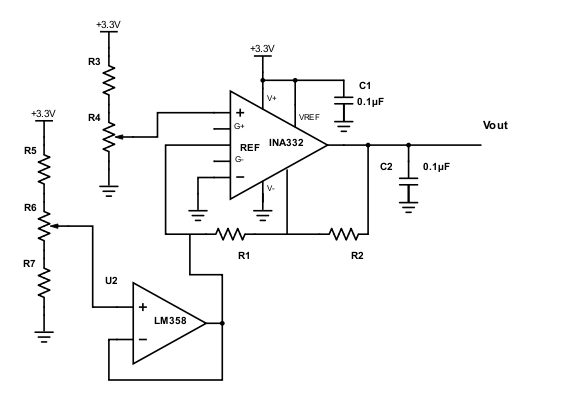
\includegraphics[width=\textwidth]{INA332-Test-Circuit}
	\caption{INA332 Test Circuit}
	\label{fig:INA332_Test_Circuit}
\end{figure}

\noindent The INA332 instrumentation amplifier is used to measure the force applied to a load cell. The amplification of this amplifier is given from the datasheet as Equation \ref{eqn:ina332-gain}. Since the load cell needed an amplification of at least 100, the calculated resistances were $R_1$ = 10k$\Omega$ and $R_2$ = 195k$\Omega$. The actual values selected for $R_1$ and $R_2$ were 10k$\Omega$ and 200k$\Omega$, respectively. This gives the amplifier an expected gain of ~105 V/V. See Figure \ref{fig:INA332_Test_Circuit} for the circuit diagram.

\begin{equation}
G = 5 + 5(\frac{R_1}{R_2})
\label{eqn:ina332-gain}
\end{equation}

\noindent The INA332 needs a voltage reference to use as the 0V differential output. Initially, two 1k$\Omega$ resistors were used to apply this voltage. This caused the output to change nonlinearly with the input voltage. The resistors were replaced with a LM358 dual operational amplifier, configured as a voltage buffer with the input connected to a potentiometer. The INA332 inputs were connected to ground and the LM358 buffer potentiometer was adjusted to set the 0V output to  $\frac{1}{2} V_{cc}$. This voltage was 1.846V. Instead of a potentiometer, two resistors were used to create this 1.846V offset.

\subsubsection{Hall Effect Encoder}
An Arduino Uno was used to ensure that the AS5055a absolute Hall effect encoder was functioning as we intended. Arduino makes rapid prototyping very easy by providing many libraries and a simple interface to quickly test a device without worrying about the board not functioning. Using the Arduino SPI library, the correct packets to send to the AS5055a were verified, along with the correct speed of both the SCLK and CS lines. The AS5055a datasheet specifies that the chip needs to receive a joint angle request at least every 0.6ms in order for the device to not go into low power mode. With this in mind, a sampling speed of 1kHz was selected.

\noindent In addition to the Arduino testing, tests were run with the TM4C123GH6PM and a test rig. The encoder test rig underwent significant revision to improve its reliability and accuracy in position the magnet above the hall effect sensor. The first iteration can be seen in Figure \ref{fig:First Iteration of Encoder Test Rig} and the second iteration can be seen in Figures \ref{fig:Second Iteration of Encoder Test Rig, Magnet View} and \ref{fig:Second Iteration of Encoder Test Rig, Side View}.

\begin{figure}[H]
	\centering
	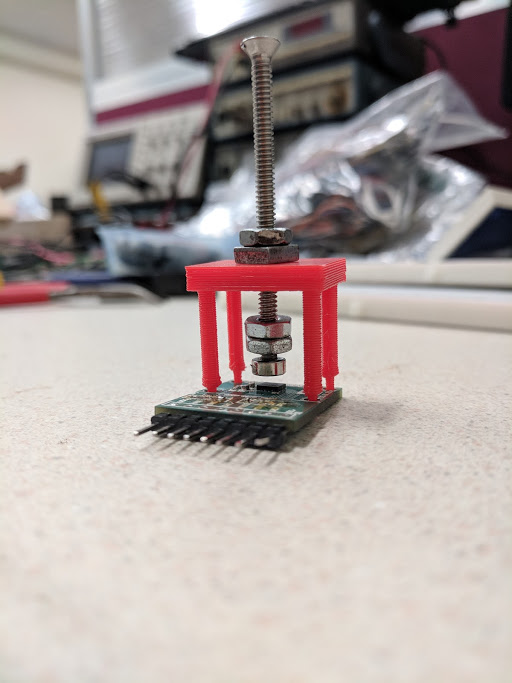
\includegraphics[scale=0.35]{encoderTestRig1}
	\caption{First Iteration of Encoder Test Rig}
	\label{fig:First Iteration of Encoder Test Rig}
\end{figure}


\begin{figure}[H]
	\centering
	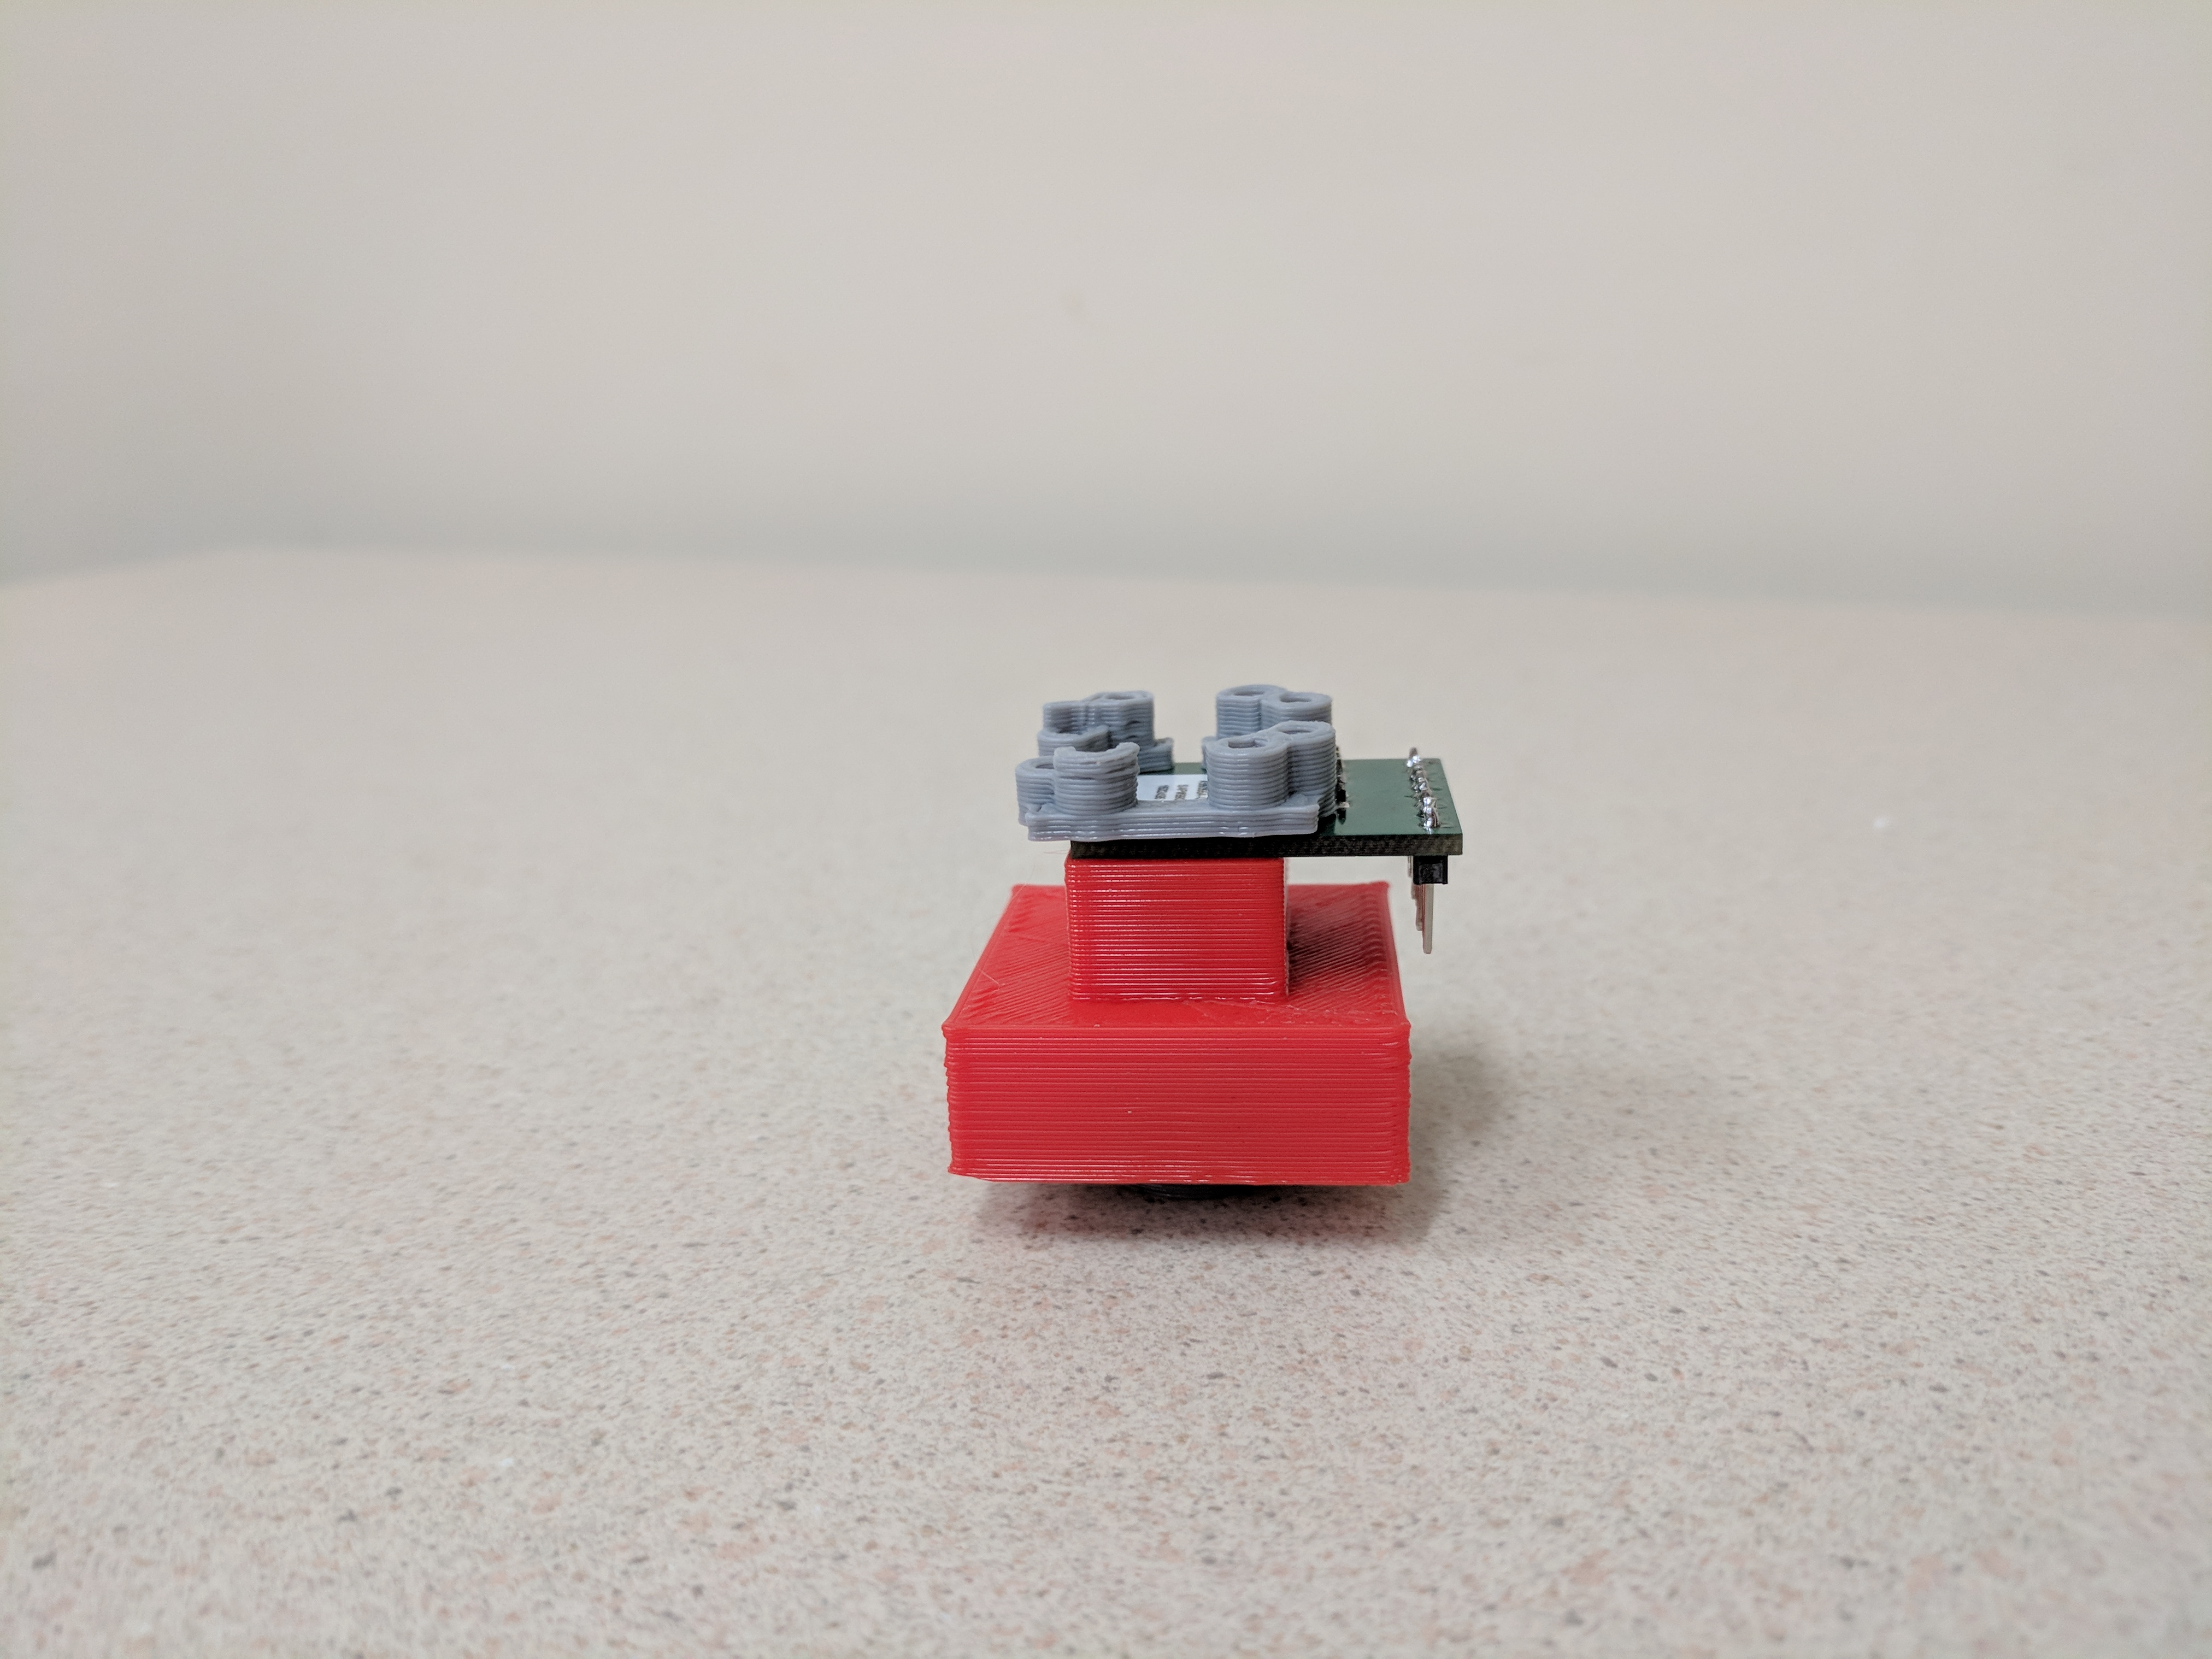
\includegraphics[scale=0.06]{hallEffect2side}
	\caption{Second Iteration of Encoder Test Rig, Side View}
	\label{fig:Second Iteration of Encoder Test Rig, Side View}
\end{figure}

\begin{figure}[H]
	\centering
	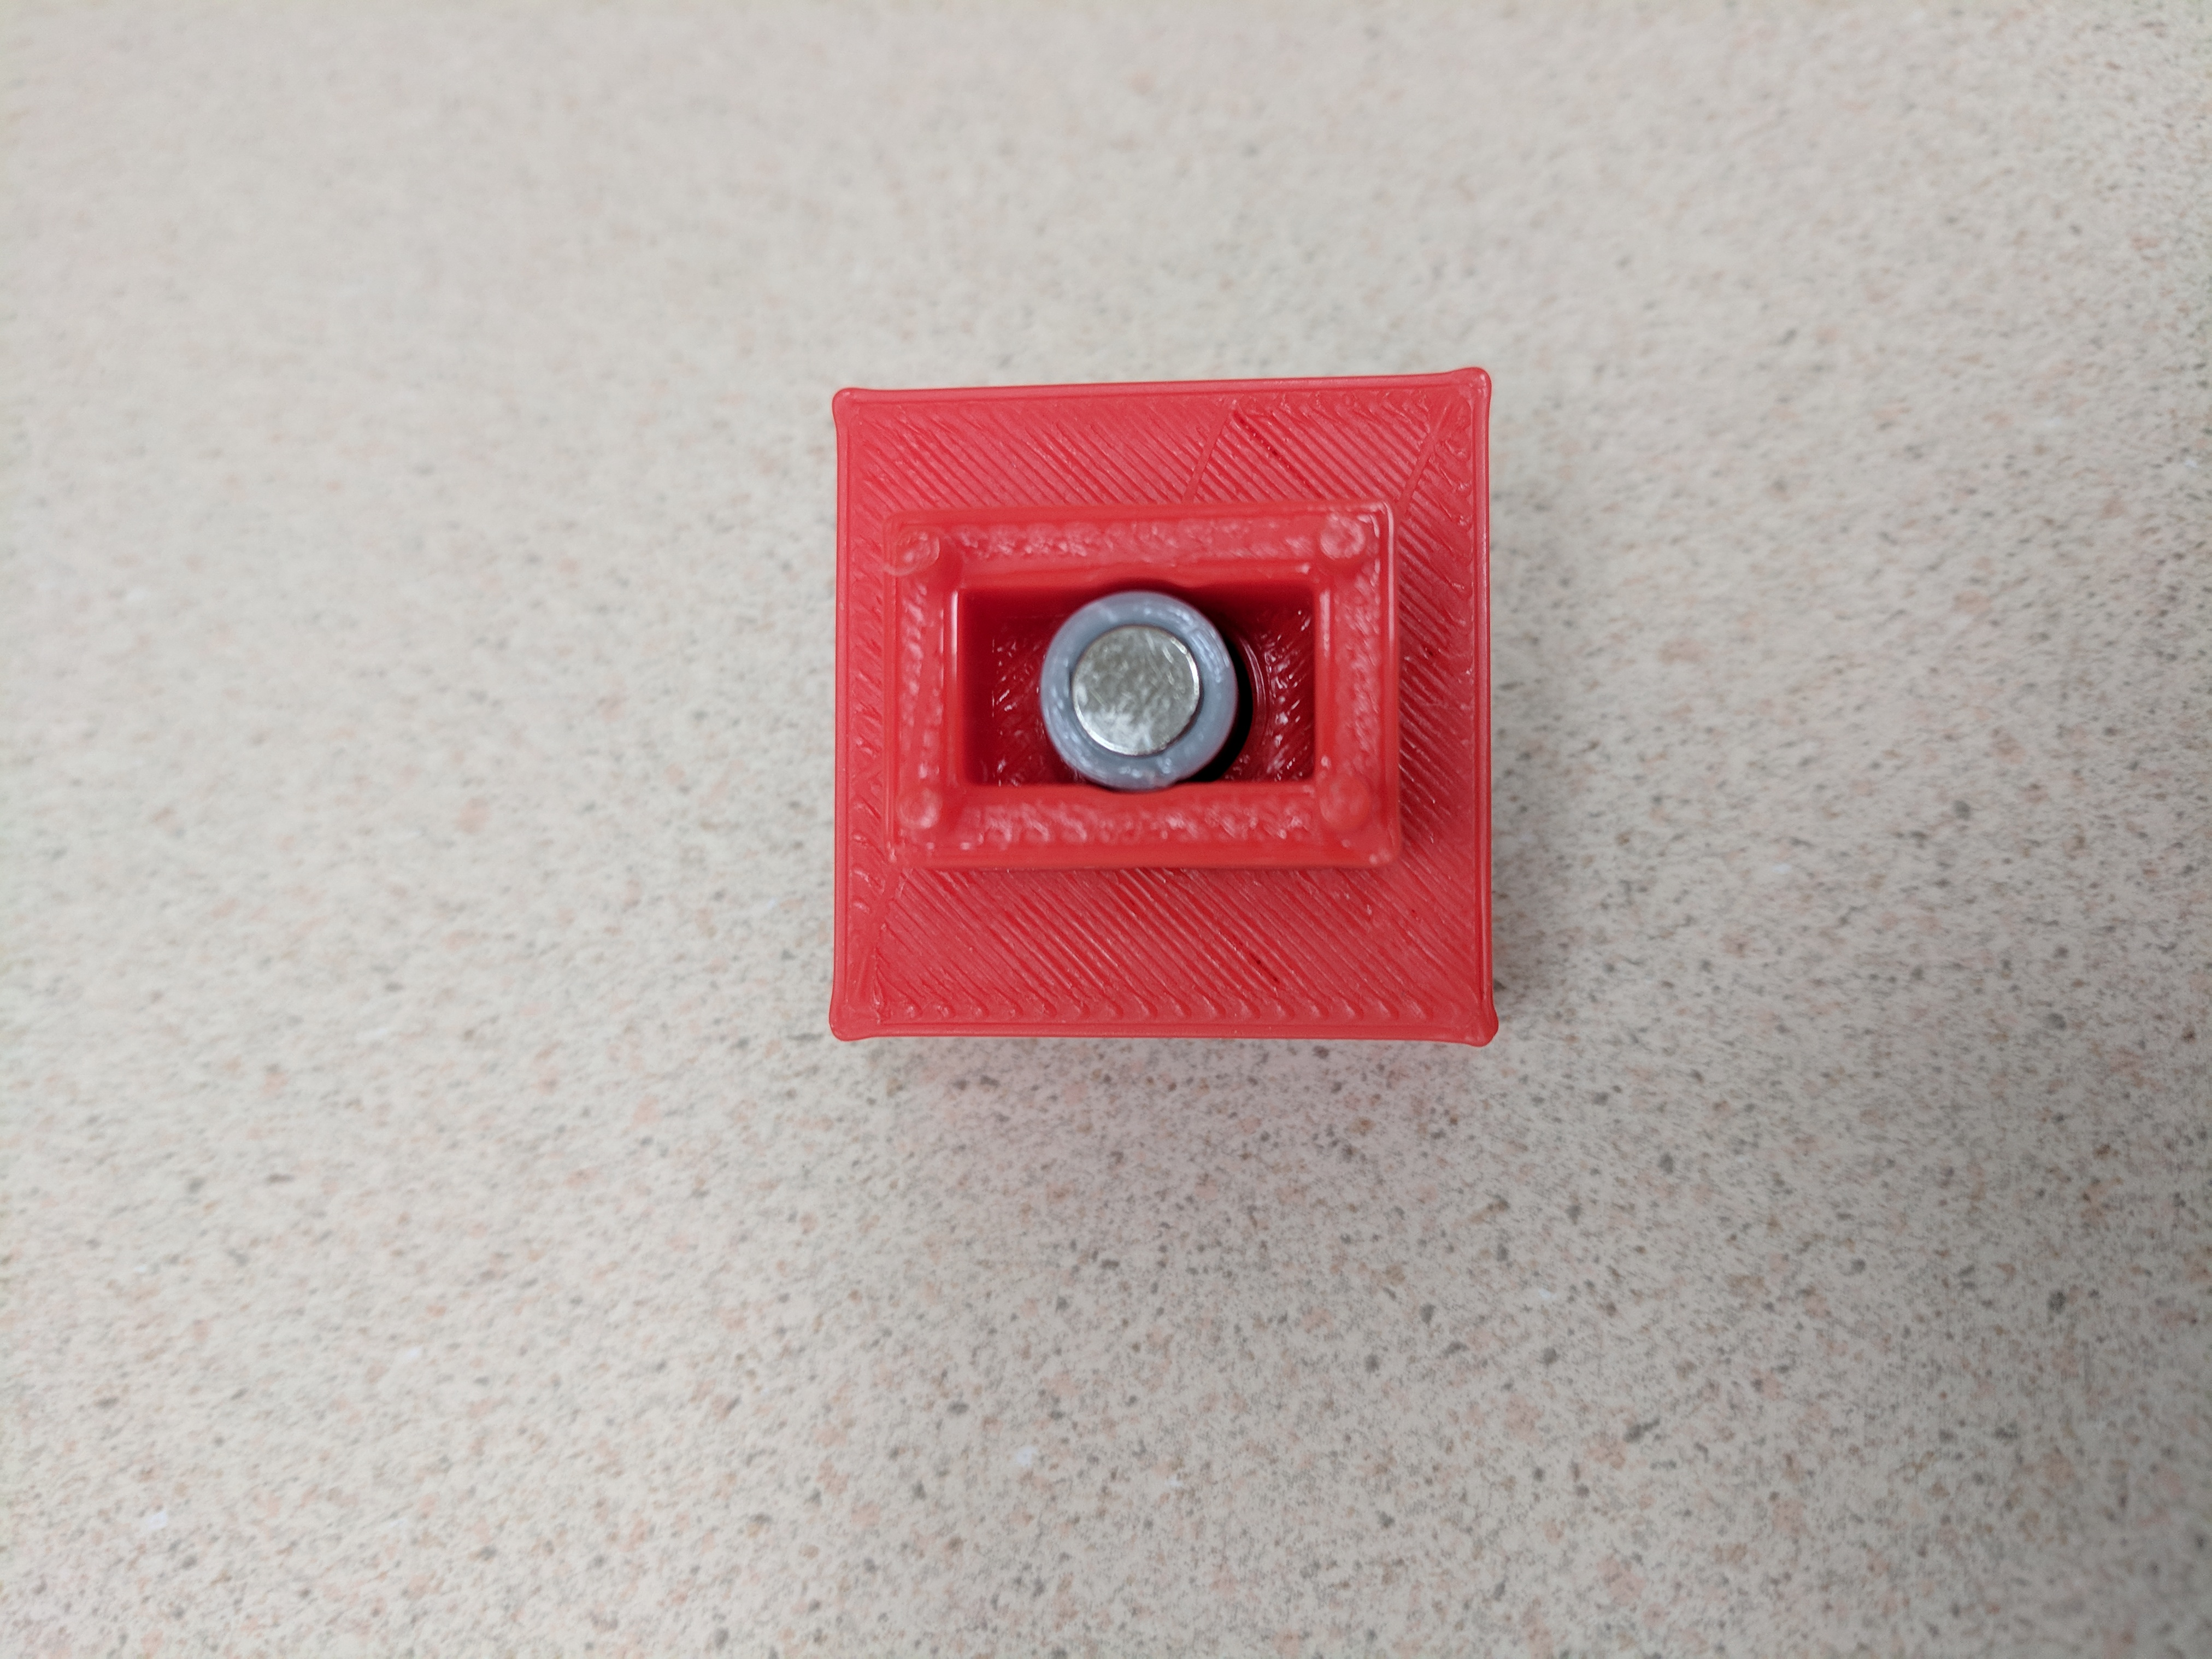
\includegraphics[scale=0.06]{hallEffect2Top}
	\caption{Second Iteration of Encoder Test Rig, Magnet View}
	\label{fig:Second Iteration of Encoder Test Rig, Magnet View}
\end{figure}

\noindent One major problem encountered with the hall effect encoder was very noisy signals. Every so often, the encoder would read a value that was around 100 counts off of all the other values read in. This is most likely either an issue with magnet alignment or a noisy SPI line. In either case, this was largely solved in code with an 8-item circular buffer and exponential filter with alpha of 0.85. Using these two in conjunction with one another, these sporadic errors were largely evened out. The value 0.85 was decided on by testing the various values. 

\noindent An alpha of 0.8 would very occasionally have erroneous readings and an alpha of 0.9 was very steady, but had a slightly delayed reaction time compared to an alpha of 0.8. An alpha of 0.85 was a compromise between steadiness and reaction time. All of the data was plotted and can be seen in Figures \ref{fig:constPosition_0_5}, \ref{fig:constPosition_0_6}, \ref{fig:constPosition_0_7}, \ref{fig:constPosition_0_8}, and \ref{fig:constPosition_0_9}.

\begin{figure}[H]
	\centering
	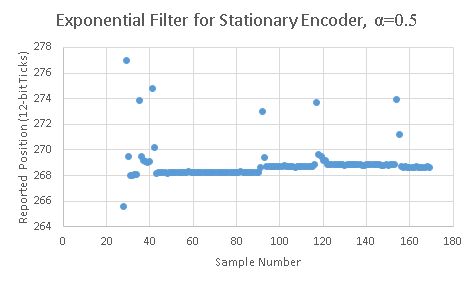
\includegraphics[scale=1.1]{constPosition_0_5}
	\caption{Behavior of the encoder value with alpha of 0.5}
	\label{fig:constPosition_0_5}
\end{figure}

\begin{figure}[H]
\centering
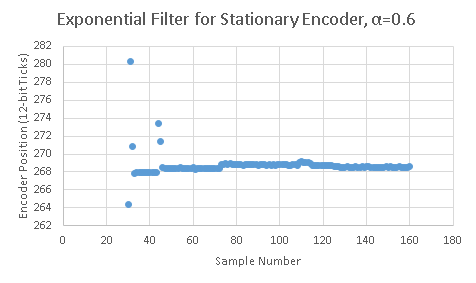
\includegraphics[scale=1.1]{constPosition_0_6}
\caption{Behavior of the encoder value with alpha of 0.6}
\label{fig:constPosition_0_6}
\end{figure}

\begin{figure}[H]
\centering
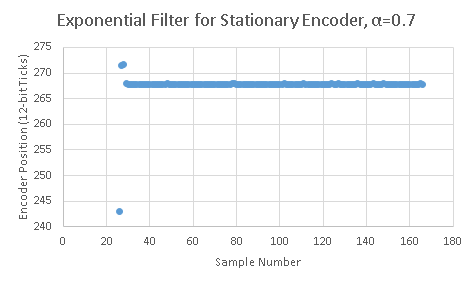
\includegraphics[scale=1.1]{constPosition_0_7}
\caption{Behavior of the encoder value with alpha of 0.7}
\label{fig:constPosition_0_7}
\end{figure}

\begin{figure}[H]
\centering
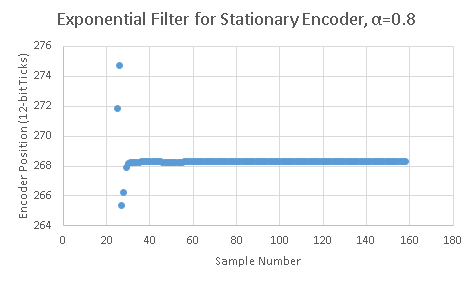
\includegraphics[scale=1.1]{constPosition_0_8}
\caption{Behavior of the encoder value with alpha of 0.8}
\label{fig:constPosition_0_8}
\end{figure}

\begin{figure}[H]
\centering
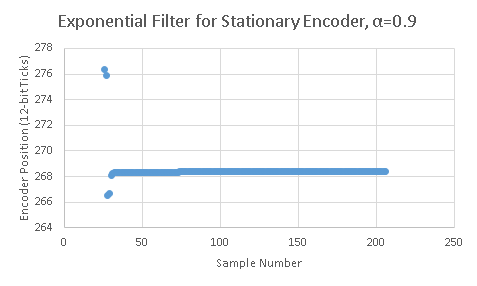
\includegraphics[scale=1.1]{constPosition_0_9}
\caption{Behavior of the encoder value with alpha of 0.9}
\label{fig:constPosition_0_9}
\end{figure}

\subsubsection{TM4C123GXL Launchpad}
Selecting a microcontroller was a key part of making the joint control board. Without a capable MCU, the joint board would not be able to function as we want it to, but buying the best microcontroller on the market can be costly. The EK-TM4C123GXL is an ARM Coretex M4f-based microcontroller evaluation kit from TI that has many peripherals to allow us to control the joint board without buying many external peripherals. The perihperals on this chip that we will need include a CAN controller, 12-bit ADC, USB controller, SSI controller, PWM controller, and many GPIO. These perihperals were implemented separately with a test circuit configured to verify that each peripheral was functioning correctly.

\noindent Several peripherals were needed to achieve the desired functionality from our microcontroller. A test board was set up in order to test and verify that each of these peripherals was setup properly and working as expected. The test board consisted of a potentiometer connected to an ADC pin, an SPI controlled ADC (MCP3202), the 1:2 demultiplexer (SN74LVC1G18), CAN transceiver (TC332), and some LEDs.

\noindent As a temporary stand in for the AS5055 absolute Hall effect encoder to test the SSI peripheral, a MCP3202 12-bit, 2 channel ADC was used. Both devices use SPI to communicate their sensor data back to the MCU, and the packets are similar in structure. Some differences between the two that can be changed are a maximum sample rate for the AS5055 of ~1ms as opposed to the few SCLK cycle delays for the MCP3202. The AS5055 has a maximum SCLK frequency of up to 10MHz at 3.3V while the MCP3202 has a limit of 900kHz at 3.3V. 

\noindent The potentiometer was connected to PE0 which was enabled at AIN3. The ADC was set to sample at 1kHz with hardware oversampling 16x enabled. A timer was configured to start an ADC conversion every millisecond, and a GPIO pin was set to 0 every time the ADC finished a conversion and set to 1 when the ADC conversion began. The time necessary to sample once at 16x hardware oversampling was around 5$\mu$s.

\subsubsection{Printed Circuit Boards}
A PCB was made for each of the major subsystems as a more final test. The subsystems for which a PCB was designed include the motor driver (both with and without a current sensor), load cell amplifier, CAN transceiver, and TM4C123GH6PM microcontroller. After these were verified to be working, a Boosterpack compatible design of the whole joint control board.

\noindent The motor driver PCB can be seen in Appendix \ref{app:motor_driver} and has the demultiplexer and a shunt resistor for triggering the automatic internal shutoff if the current gets too high. The motor driver with current sensor has a current sensor integrated in the board and can be seen in Appendix \ref{app:motor_driver_current}. The load cell amplifier has the LM358 op amp as well as the INA332 instrumentation amplifier and can be seen in Appendix \ref{app:load_cell_amp}. The CAN transceiver PCB was designed that contains the 6 necessary DIP switches, CAN transceiver, and auto-terminate circuit and can be seen in Appendix \ref{app:can_transceiver}. The joint control board Boosterpack has all of these components in a single PCB that mounts on top of the TM4C123GXL Launchpad and can be seen in Appendix \ref{app:joint_board_boosterpack}. All of these PCBs can be seen in Figure \ref{fig:pcbs}. A closeup of the joint control board Boosterpack attached to a Launchpad can be seen in Figure \ref{fig:jcb_boosterpack}.

\begin{figure}[H]
	\centering
	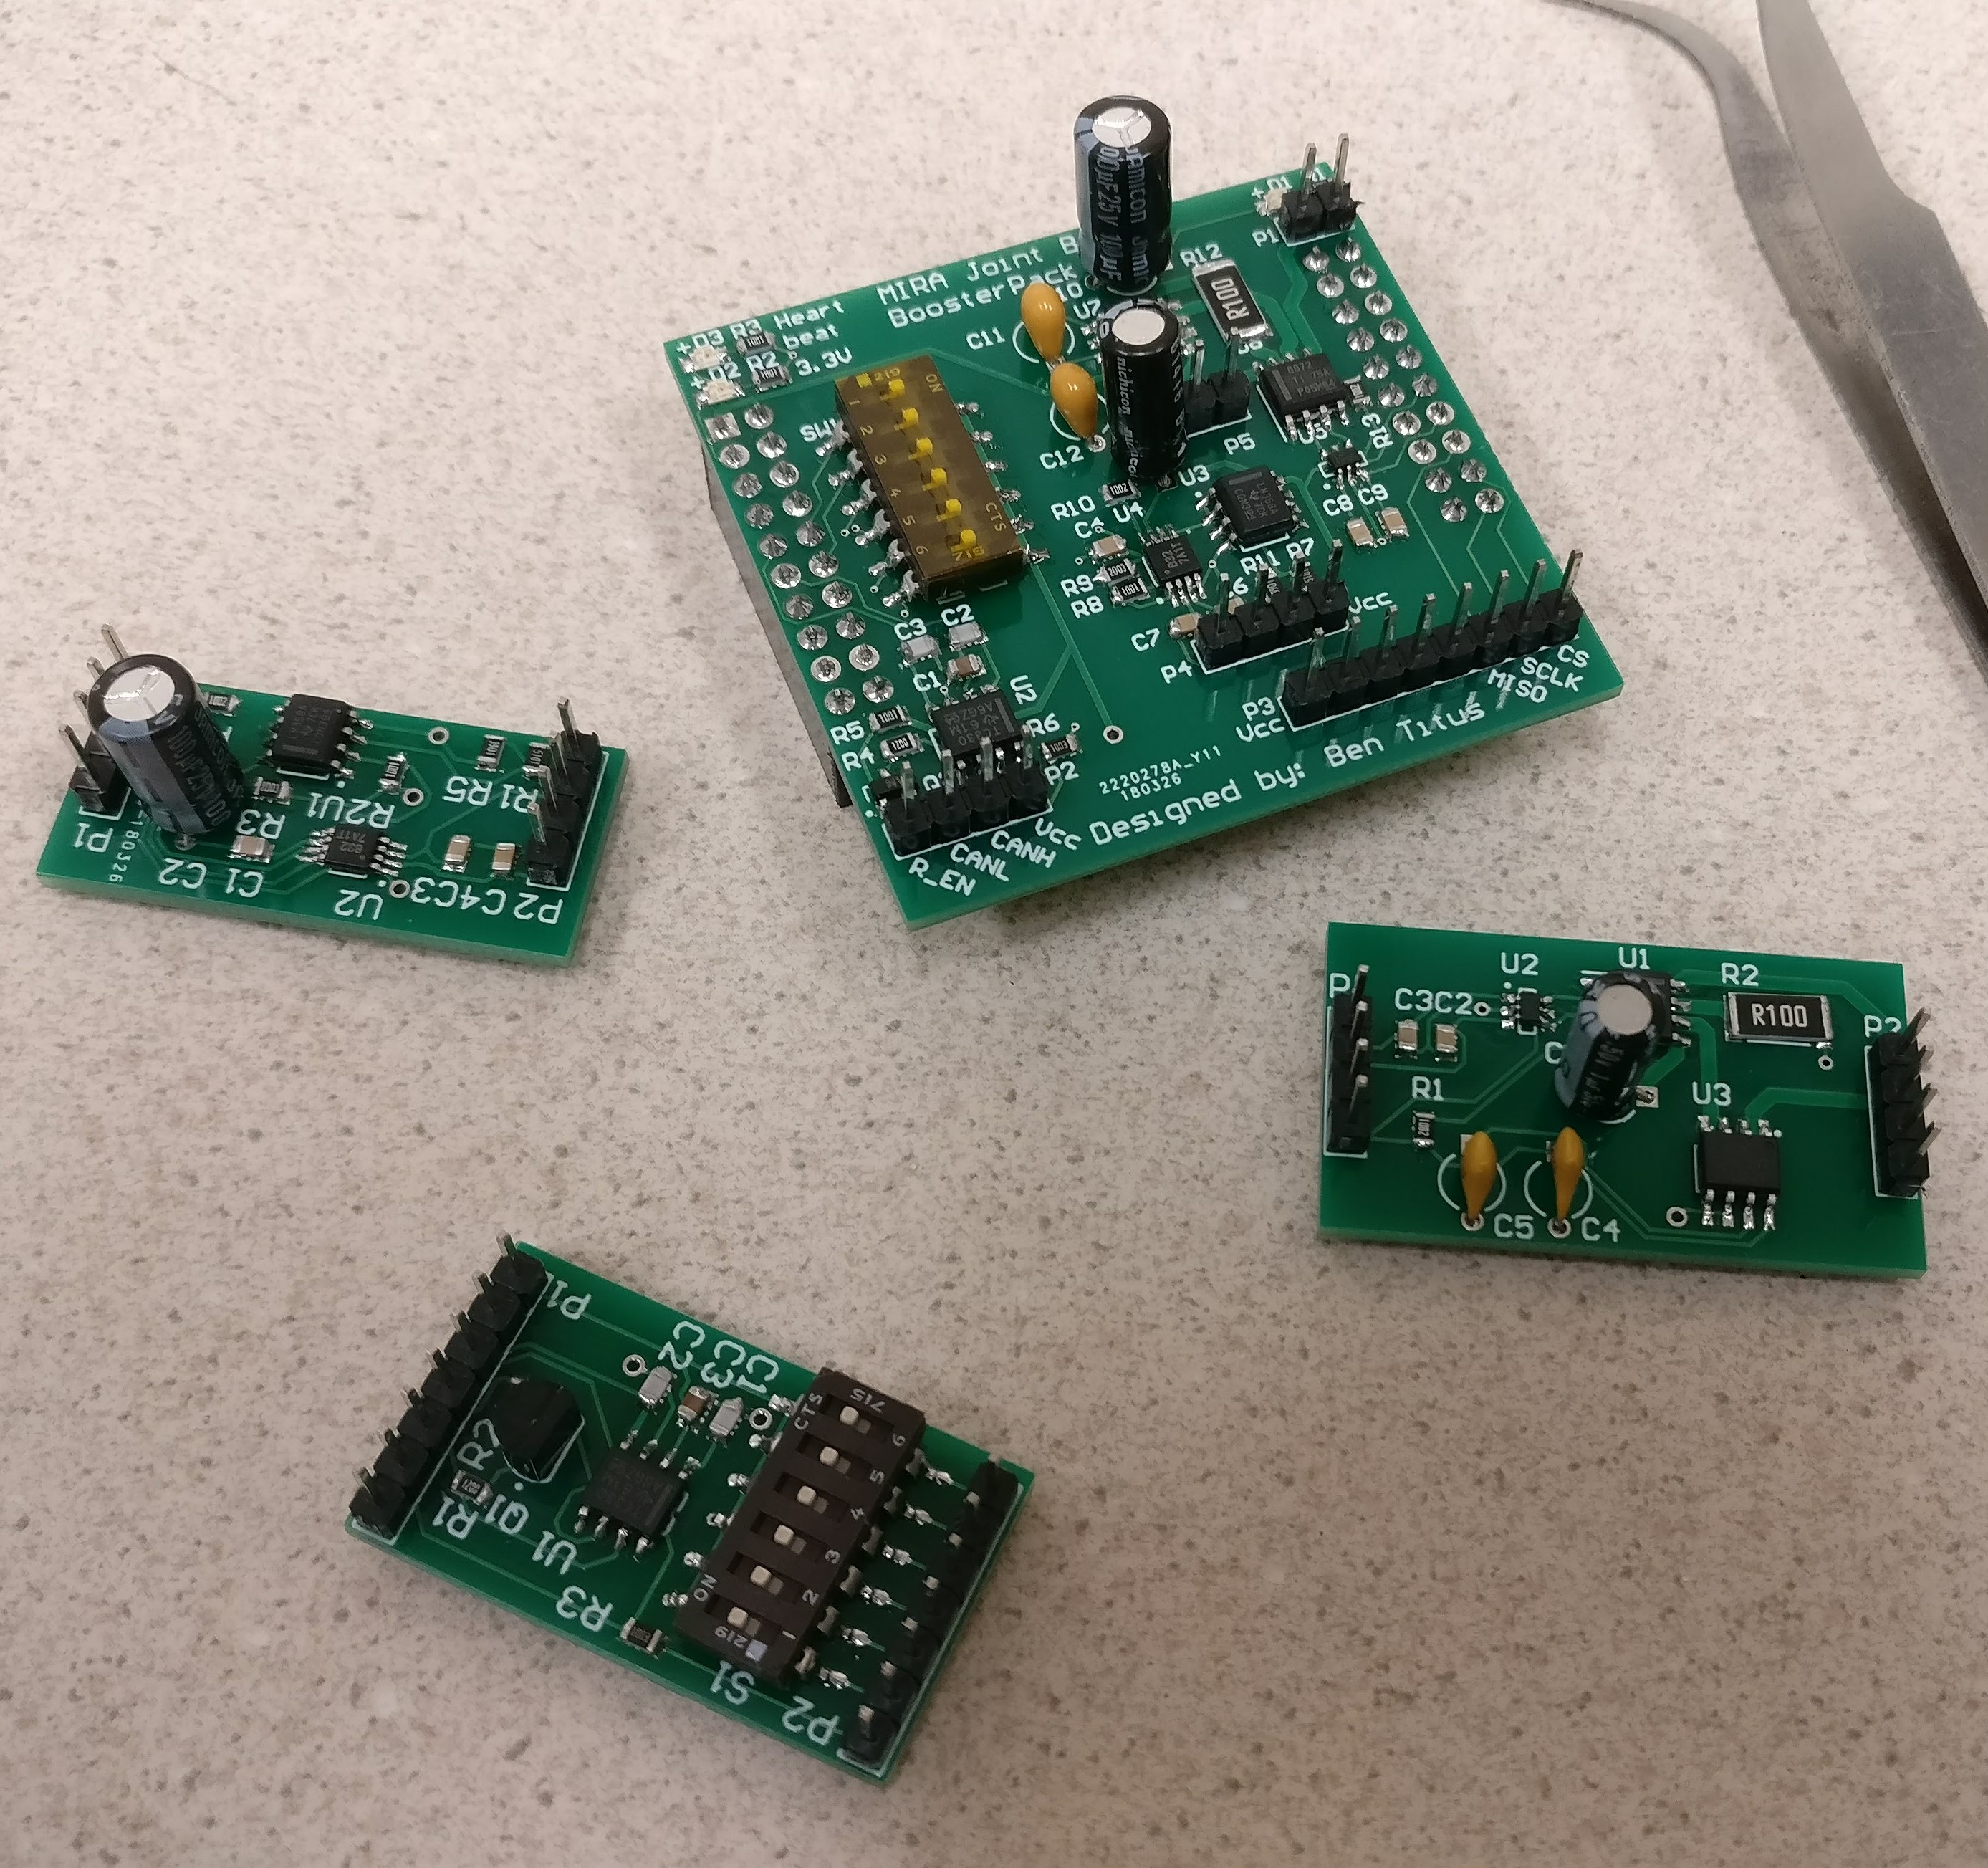
\includegraphics[scale=0.1]{pcbs}
	\caption{Assembled PCBs of each major subsystem including motor driver with current sensor (right), CAN transceiver (bottom), load cell amplifier (left), and joint control board Boosterpack (top)}
	\label{fig:pcbs}
\end{figure}

\begin{figure}[H]
	\centering
	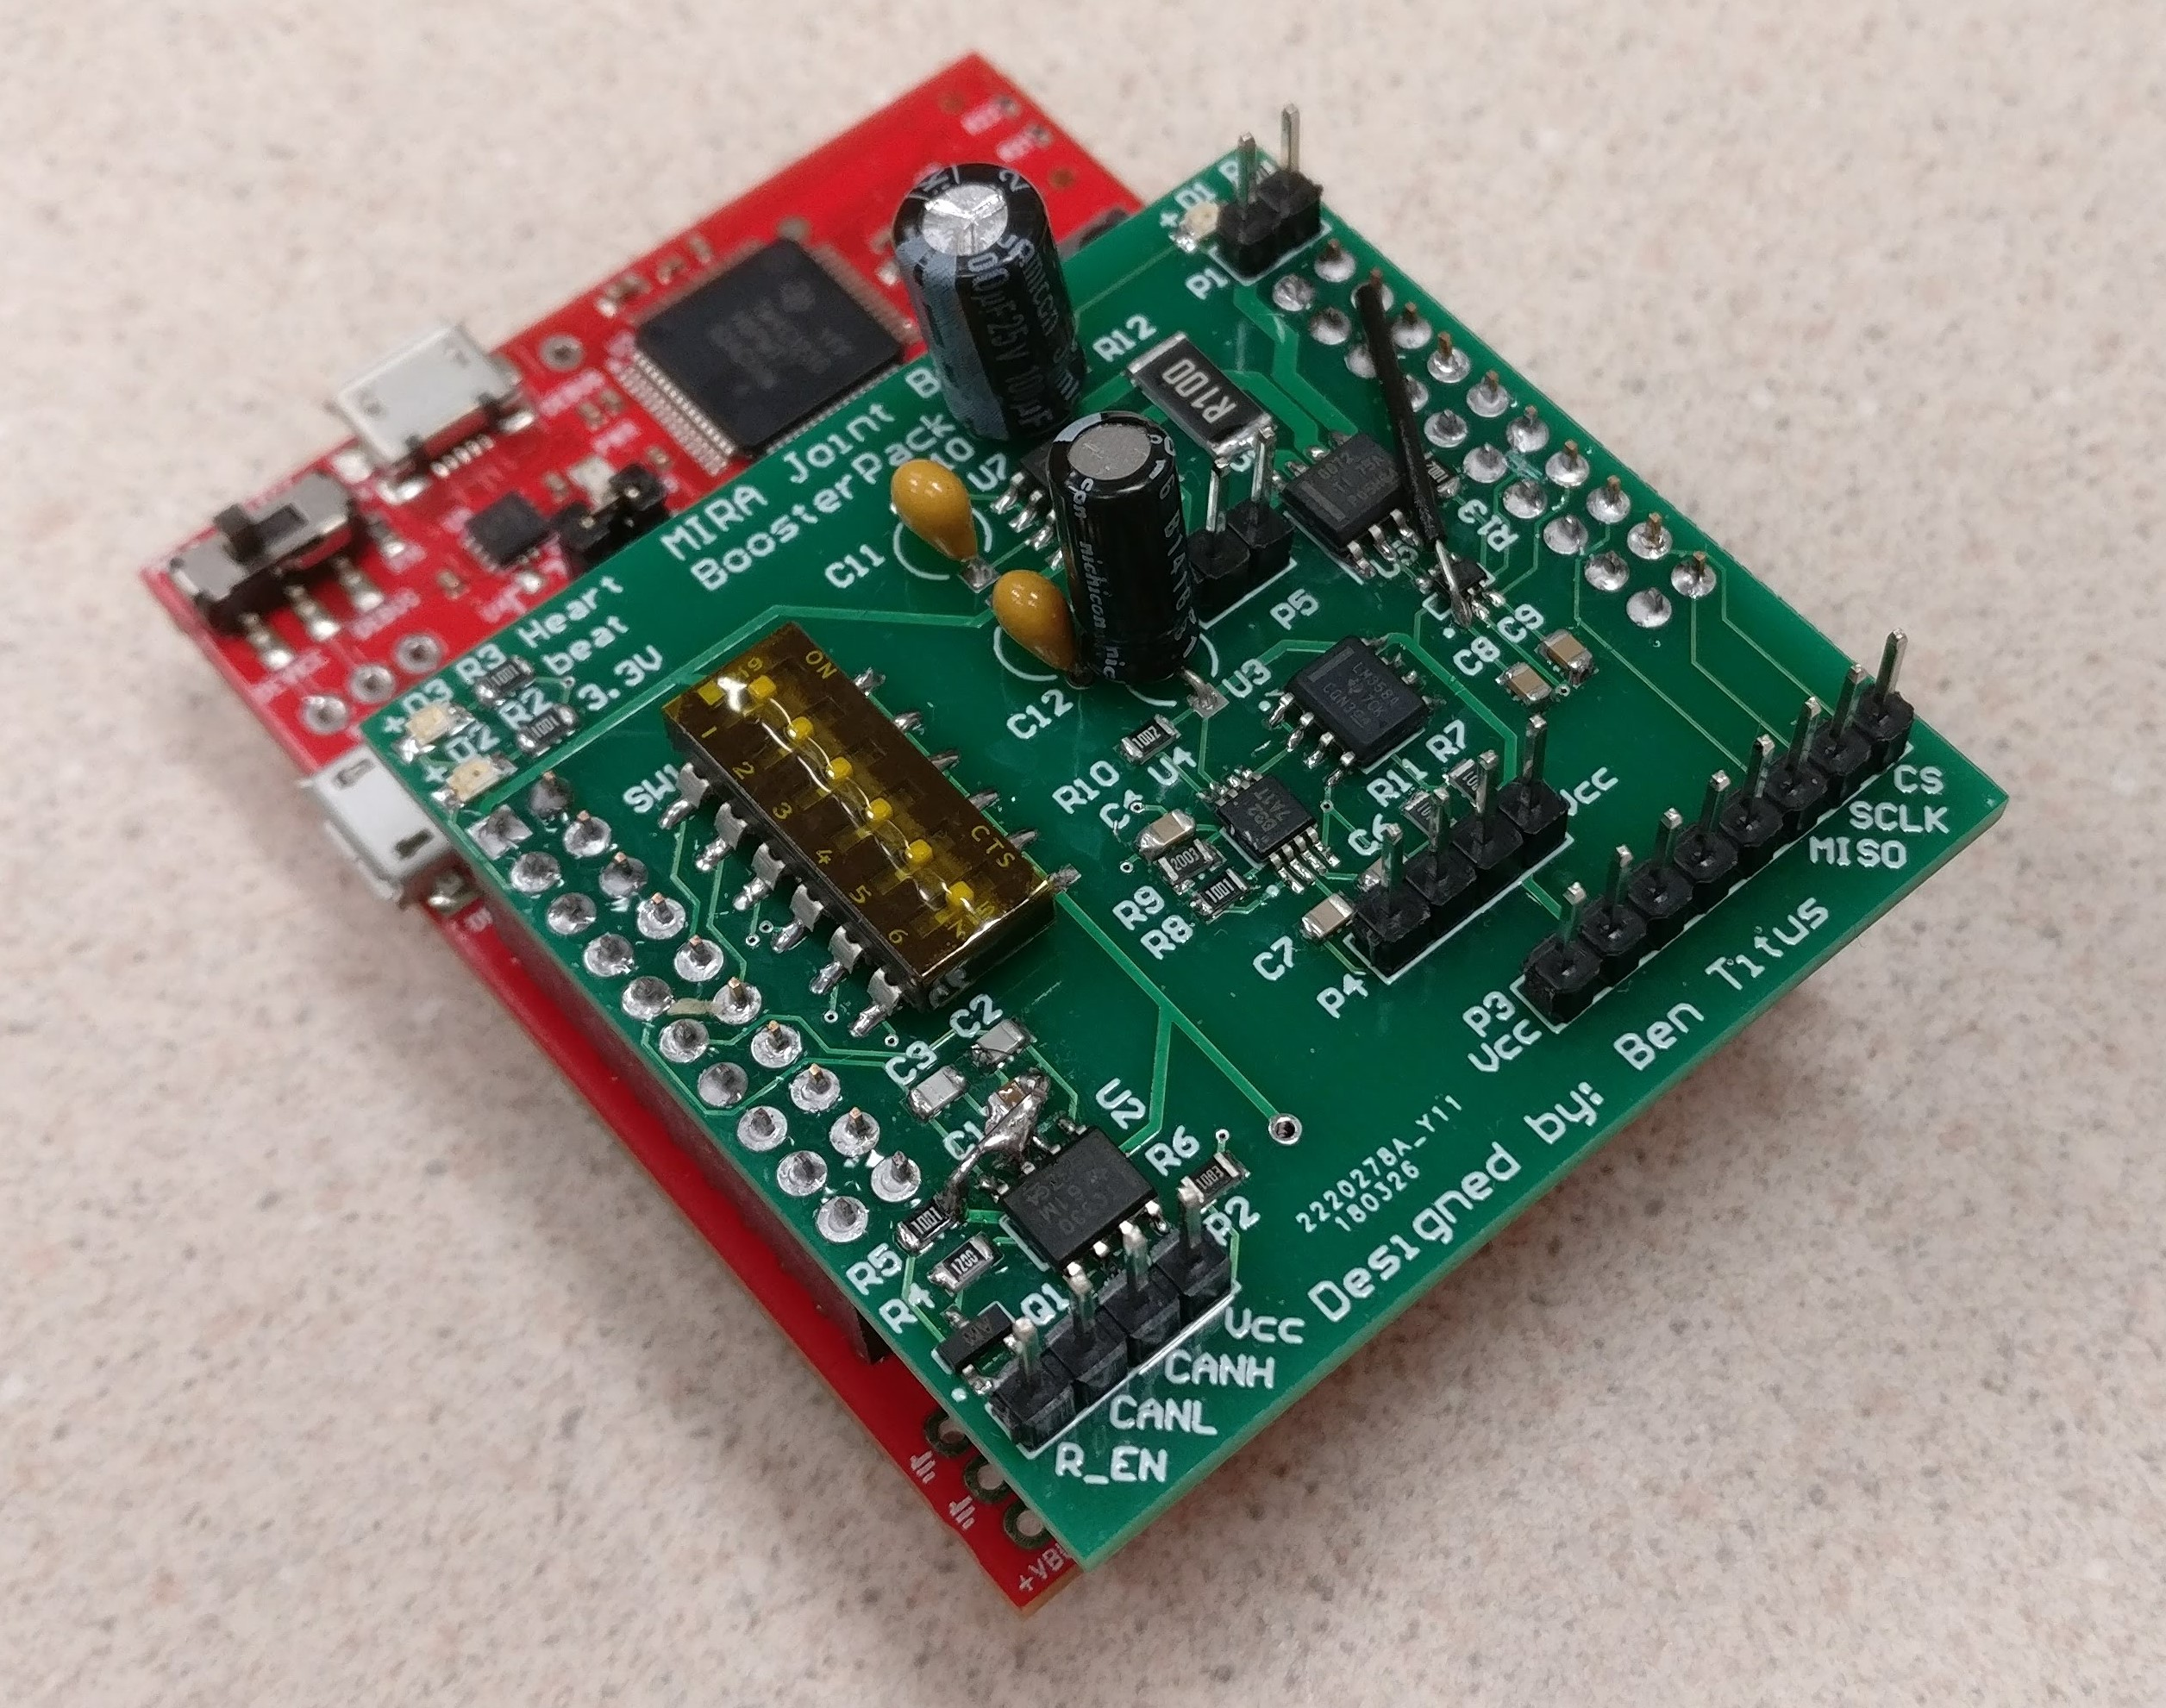
\includegraphics[scale=0.1]{jcb_boosterpack}
	\caption{Joint control board Boosterpack on the TM4C123GXL Launchpad}
	\label{fig:jcb_boosterpack}
\end{figure}

\noindent Small problems existed in some of the PCBs during the first revision. The CAN transceiver PCB has the $V_{CC}$ and GND pins swapped. Once this problem was identified, the traces were cut, wire soldered, and the schematic altered for another revision. The load cell amplifier PCB has a GND pin that was not connected to anything. The GND pin on the INA332 amplifier had an unconnected ground pin. This pin was connected with wire, and the PCB worked as expected.

\noindent The joint control board Boosterpack had the CAN transceiver $V_{CC}$ and GND pins swapped as well as needing the motor direction pin to be moved from one pin to another. This change came about due to the Launchpad construction. Two of the pins were connected internally but labeled differently, so the motor direction pin was swapped in code, the trace was cut, and wire was soldered to the new pin. These changes can be seen in Figure \ref{fig:jcb_boosterpack}. Another revision of the joint control board Boosterpack was made but not ordered due to time constraints. A repository containing all of the altium files for these PCBs can be found in Appendix \ref{app:code_repo}.

\subsubsection{Joint Control Board Code}
%TODO: talk about RTOS, put flowchart, talk about CAN challenges
The joint control board code uses TI's RTOS for TivaWare. The main reason for this decision was to gain access to the task synchronization that the RTOS provides to compartmentalize the code into different threads. A code flowchart can be seen in Figure \ref{fig:jcb_code_flowchart}. There are many threads running alongside one another, but they are all fairly separated in terms of their functionality. Each thread handles a single function, for example there is a thread for processing encoder data. This thread is released on a 1kHz software timer. The code repository can containing this code as well as a repository containing testing code can be found in Appendix \ref{app:code_repo}.

\begin{figure}[H]
	\centering
	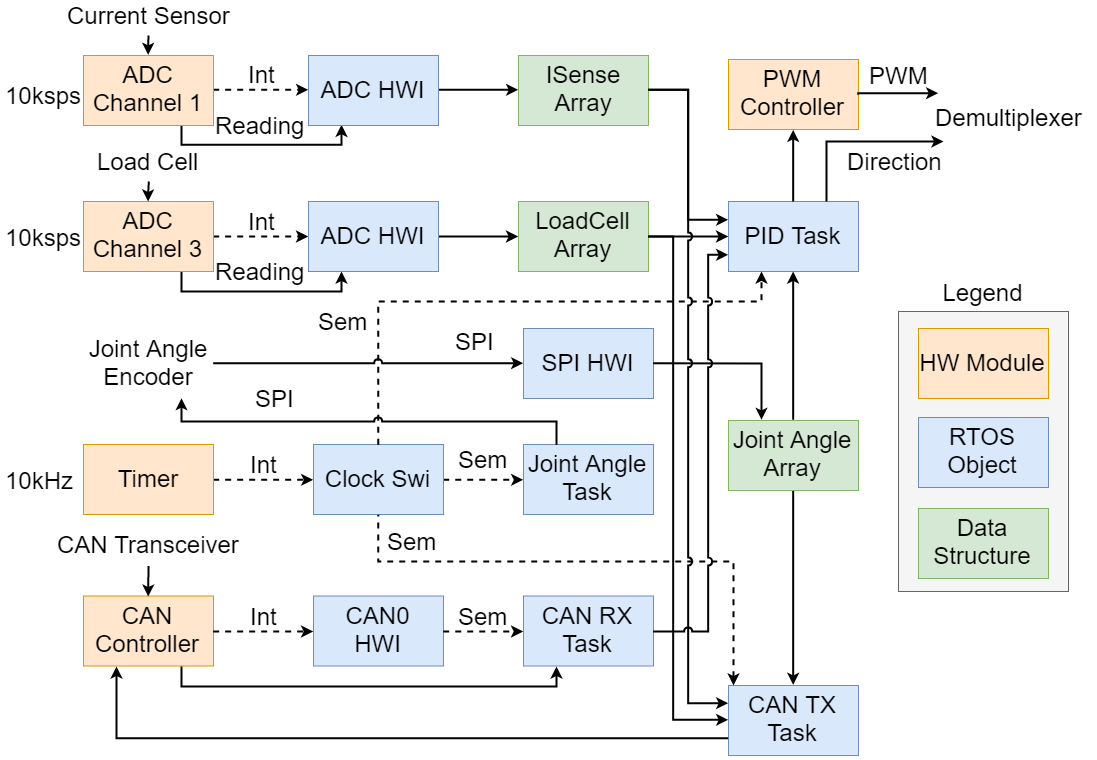
\includegraphics[scale=0.35]{jcb_code_flowchart}
	\caption{Joint control board code flowchart}
	\label{fig:jcb_code_flowchart}
\end{figure}

\subsection{CAN Bus}
The CAN bus is the spine of the control system, carrying messages from the base to each joint and back from each of the joints to the base. Unit tests and careful integration were done to ensure that this tricky protocol was implemented properly and robustly while leaving room for future implementation of additional message types.

\subsubsection{Determining Joint Placement with Message ID}
CAN bus will be used to communicate between the base and joints. A limitation of CAN is that there is no way of determining the position of a module on the bus. This is important for controlling a robot arm since joint 1 is controlled differently from joint 2, etc. In order to determine the position of a joint board on the bus, another method is needed. The CAN message ID contains 11 bits in the standard frame.

\noindent We decided to use the upper 6 bits as a joint board number identifier, a number unique to that specific joint board, and the lower 5 bits as a message type. By doing this, we can tell the base the joint identifier number and position on the arm to rout position update messages to the correct joint on the arm.

\noindent There were a few ways of accomplishing this. One would be to program each joint board with a different identifier number. This could get very tedious and confusing for having many joint boards, since we would have to change and track identifier numbers for each unique joint board. Another option was to use EEPROM to automatically store the identifier number and upload it via the USB cable used for programming the board. This could get complicated since we would have to write code to not only read in the identifier properly, but also store it in EEPROM properly. Instead, we decided to use DIP switches. DIP switches allow us to input the identifier number in binary and update them on the fly without reprogramming the board.

\begin{figure}[H]
\centering
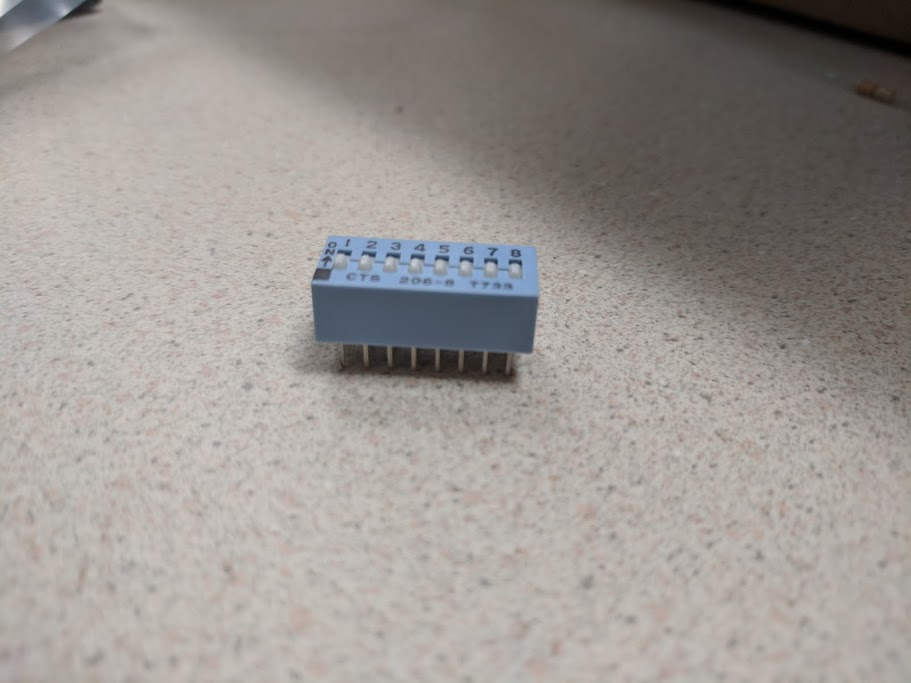
\includegraphics[scale=0.2]{cuteDipSwitch}
\caption{8-channel DIP Switch}
\label{fig:8_channel DIP Switch}
\end{figure}

\noindent On startup, the joint board reads in the identifier bits and stores them in a variable. The identifier is then used as a mask for the CAN message receive IDs. The CAN controller compares incoming message IDs to the ID mask and ID value set when initializing the message receive object. When setting the message receive object, we can set the message ID to the joint board identifier, shifted up by 5 bits, and set the mask to only listen for messages that match the upper 6 bits. We can set the message receive object to receive messages with the joint board ID in the upper 6 bits, regardless of message type. Since there are 32 message objects available on the CAN controller of the TM4C123GH6PM microcontroller, we have a great amount of flexibility for listening to different types of messages.

\begin{table}
	\centering
	\caption{CAN message ID breakdown}
	\begin{tabular}{| c | c |}
		\hline
		CAN ID & Message type \\
		\hline
		\textsc{000000XXXXX} & Reserved \\
		\textsc{XXXXXX00000} & Init Encoder \\
		\textsc{XXXXXX00001} & Init PID P constant \\
		\textsc{XXXXXX00010} & Init PID I constant \\
		\textsc{XXXXXX00011} & Init PID D constant \\
		\textsc{XXXXXX00100} & Position update to joint \\
		\textsc{XXXXXX10000} & Position update to base\\
		\hline
	\end{tabular}
\end{table}

\subsubsection{Implementing a Simple CAN Bus}
The preliminary CAN setup consisted of two TM4C Launchpads, one with transmit code and one with receive code. The transmitting board was set up for 1Mbps transmission with message ID = 2, and message length = 1 byte. The message data was a 4-bit value that incremented every time the message was successfully transmitted. A software delay was used to slow the transmission rate down to about every ~second. The receive board was set up for 1Mbps transmission with message ID = 0, message ID mask = 0, and message length = 1 byte. Setting both the message ID and mask to 0 signals the controller to accept any message. 4 LEDs were set up to see the CAN message data visually.
%TODO: insert table of configuration data

\noindent We had several problems getting this simple example to work. Initially, one of the jumper wires used for the CAN bus was broken, causing the CAN Hi lines on the transceivers to not be connected. The next problem was that the sample code provided by TI was not correct. When the CAN controller receives a valid message, it signals the processor with an interrupt. When a receive interrupt is processed by the example code, the interrupt flag is cleared and then the message data is read in. The problem is that when the interrupt flag is cleared, the new data bit that signals that there is valid data available is cleared. To fix this, the operations must be switched so that message data is read in before the interrupt flag is cleared. Once this fix was applied, CAN communications were functional. 

\noindent During the debugging process, a logic analyzer (Saleae 8-channel logic analyzer) was used to verify correct transmission of CAN packets. The logic analyzer software can be seen in Figure \ref{fig:can_logic_analyzer} decoding a packet with ID 2, data length 1, data byte equaling 7, and a proper ACK signal. The x marks a bit that was inserted to keep the timing consistent among the transceivers. Additionally, Figure \ref{fig:can_TXD_RXD} shows the ACK bit on the RXD line (channel 2) and no ACK bit on the TXD line (channel 0).

\begin{figure}[H]
	\centering
	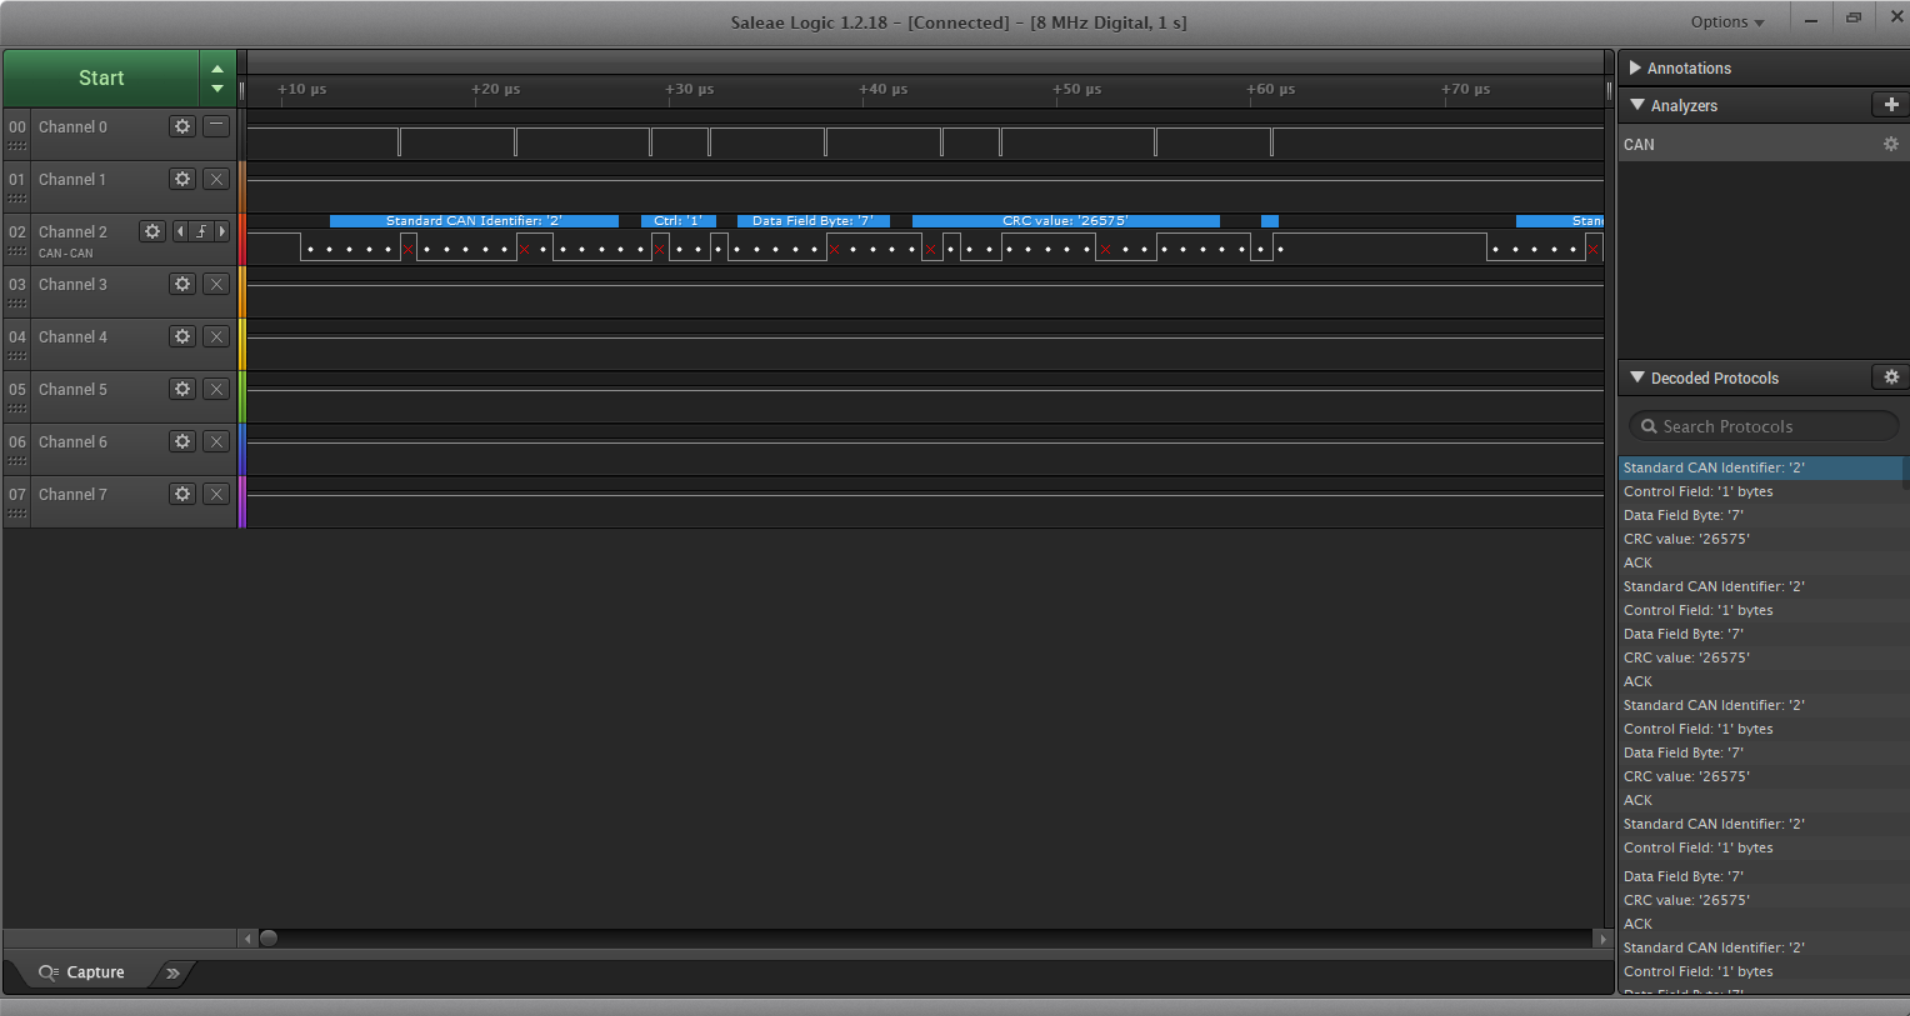
\includegraphics[width=\textwidth]{CAN_Logic_Analyzer}
	\caption{CAN bus as viewed in the logic analyzer software}
	\label{fig:can_logic_analyzer}
\end{figure}

\begin{figure}[H]
	\centering
	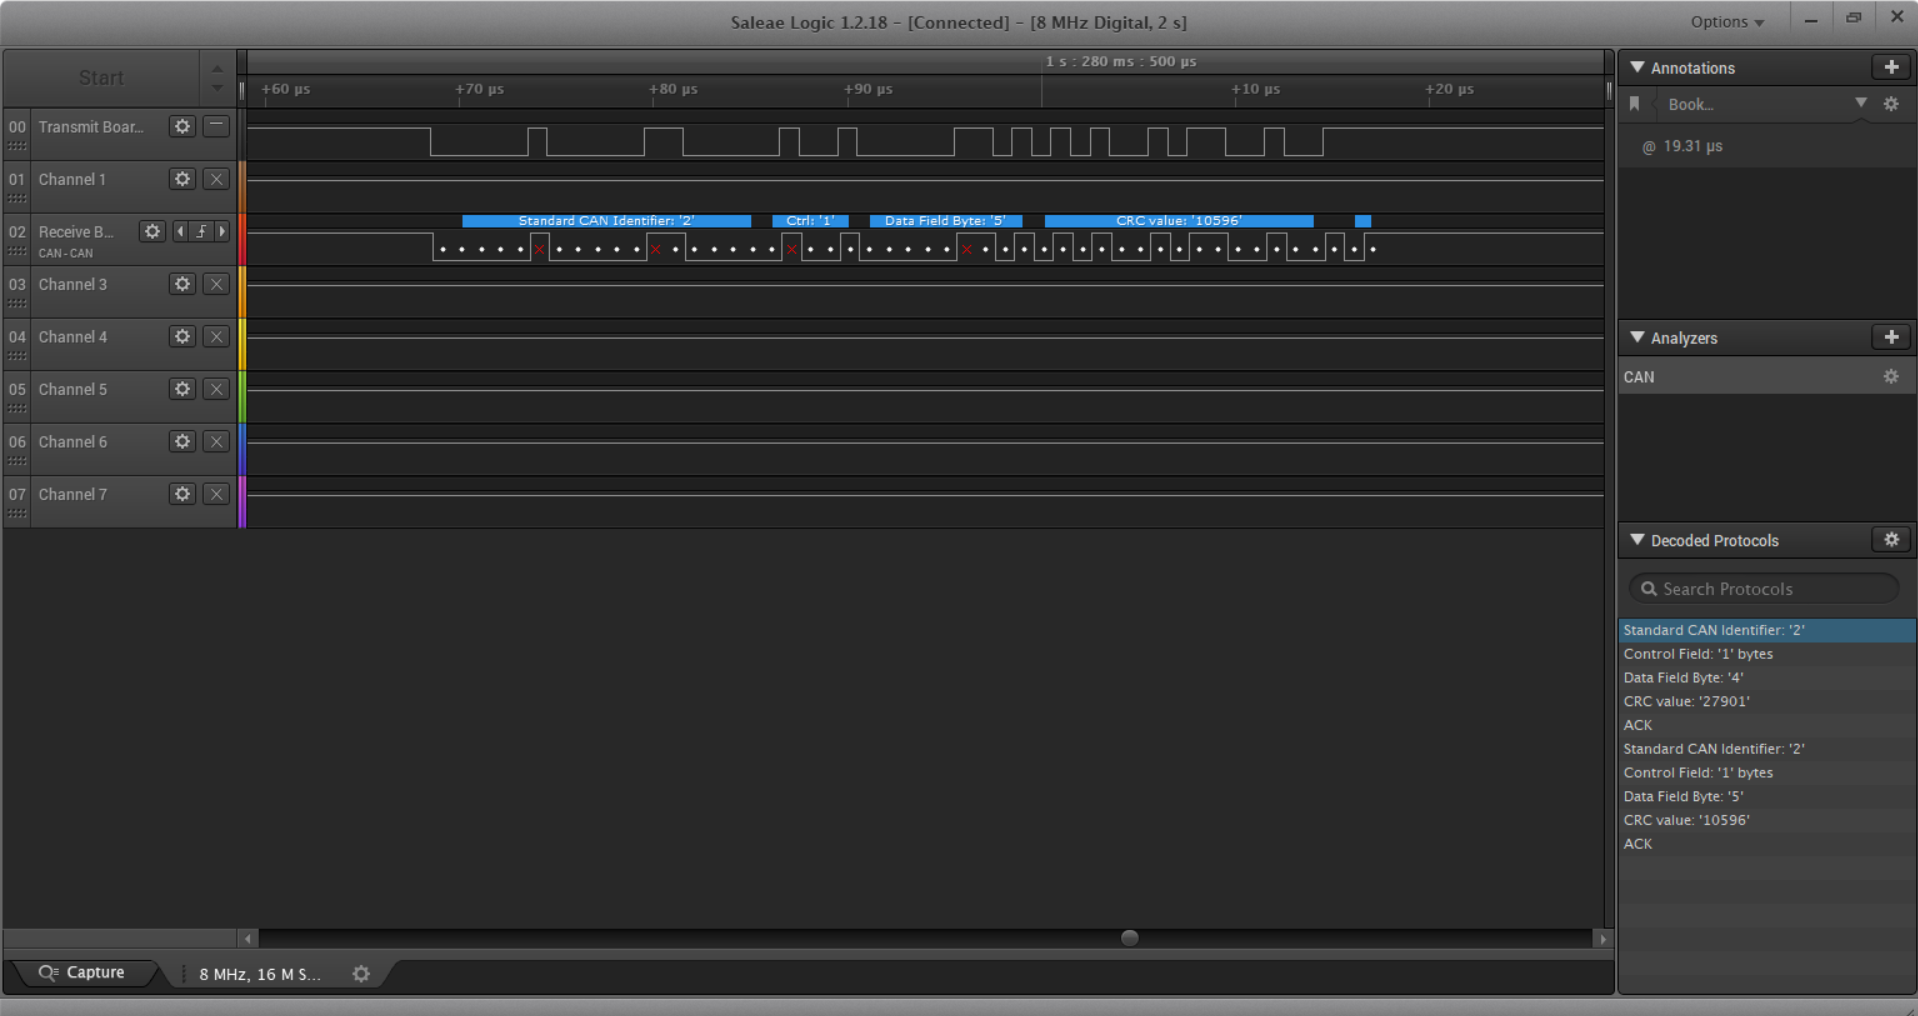
\includegraphics[width=\textwidth]{CAN_TXD_to_RXD}
	\caption{CAN TXD (channel 0) and RXD (channel 2) in the logic analyzer software}
	\label{fig:can_TXD_RXD}
\end{figure}

\subsubsection{CAN Termination}
CAN specification states that the CAN bus needs to be terminated on both ends by 120$\Omega$ resistors. The purpose of these resistors is to help mitigate signal reflections as well as pull the CAN Hi and CAN Lo lines together when the bus state is recessive. Since the resistors need to be at either end of the CAN bus, using normal resistors requires a static bus configuration. Our system will not necessarily have a fixed configuration, though, so a different solution was needed.

\noindent One method was to require the end user to attach a unique component, such as an end effector, at either end of the bus. This would effectively mean that an arm would always need a base module and an end effector to function properly. This rigid definition was not something we wanted to enforce on the end user, so instead we came up with a auto-disconnect circuit to disconnect the terminating resistor if another joint is added to the arm.

\noindent The way this works is through a MOSFET switch, seen in Figure \ref{fig:can_terminate_circ}. The MOSFET (part number BS170) drain and source connect the CAN Hi and CAN Lo lines through a 120$\Omega$ resistor and the gate is pulled up to $V_{DD}$ through a 1l$\Omega$ resistor. When the next joint is connected, the gate is connected to ground and the MOSFET is opened, disconnecting the CAN Hi and CAN Lo lines. When there is no joint connected, the MOSFET is closed, effectively acting as a 5$\Omega$ resistor in series with the 120$\Omega$ resistor. This new 125$\Omega$ resistance is within tolerance in the CAN specifications which state that the resistance must be between 50$\Omega$ and 70$\Omega$.

\begin{figure}[H]
	\centering
	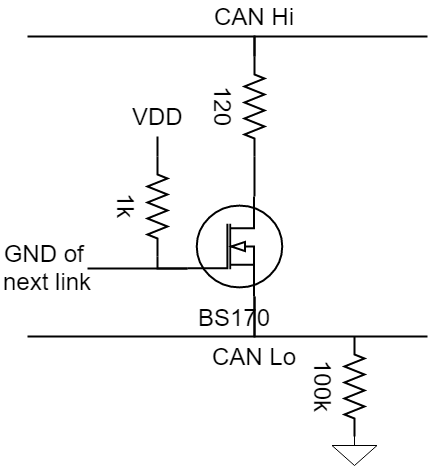
\includegraphics[scale=0.5]{CAN_terminate}
	\caption{CAN bus auto-terminate circuit}
	\label{fig:can_terminate_circ}
\end{figure}

\subsubsection{Position Updates}
The control system supports up to 6 joints at a time. In order to have a constant transmission speed for every combination of joints up to and including 6 joints, 6 joint update packets are sent every update. When fewer than 6 joints are used, the remaining packets are transmitted but never received. This is one place where using the CAN bus helps, since these messages don't need to be received by a specific receiver. Only the ACK bit needs to be sent when no errors are detected with packet structure, but this can be sent by any received. 

\noindent Since all 6 joints were being updated every time, the minimum update time is the time it takes to transmit 6 CAN packets. This time was measured to be about 0.8ms with a transmission speed of 500kHz using the logic analyzer and can be seen in Figure \ref{fig:can_joint_update}. The joint update and response were both sent at a rate of 20Hz, 50ms apart, and can be seen in figure \ref{fig:can_joint_update_response}.

\begin{figure}[H]
	\centering
	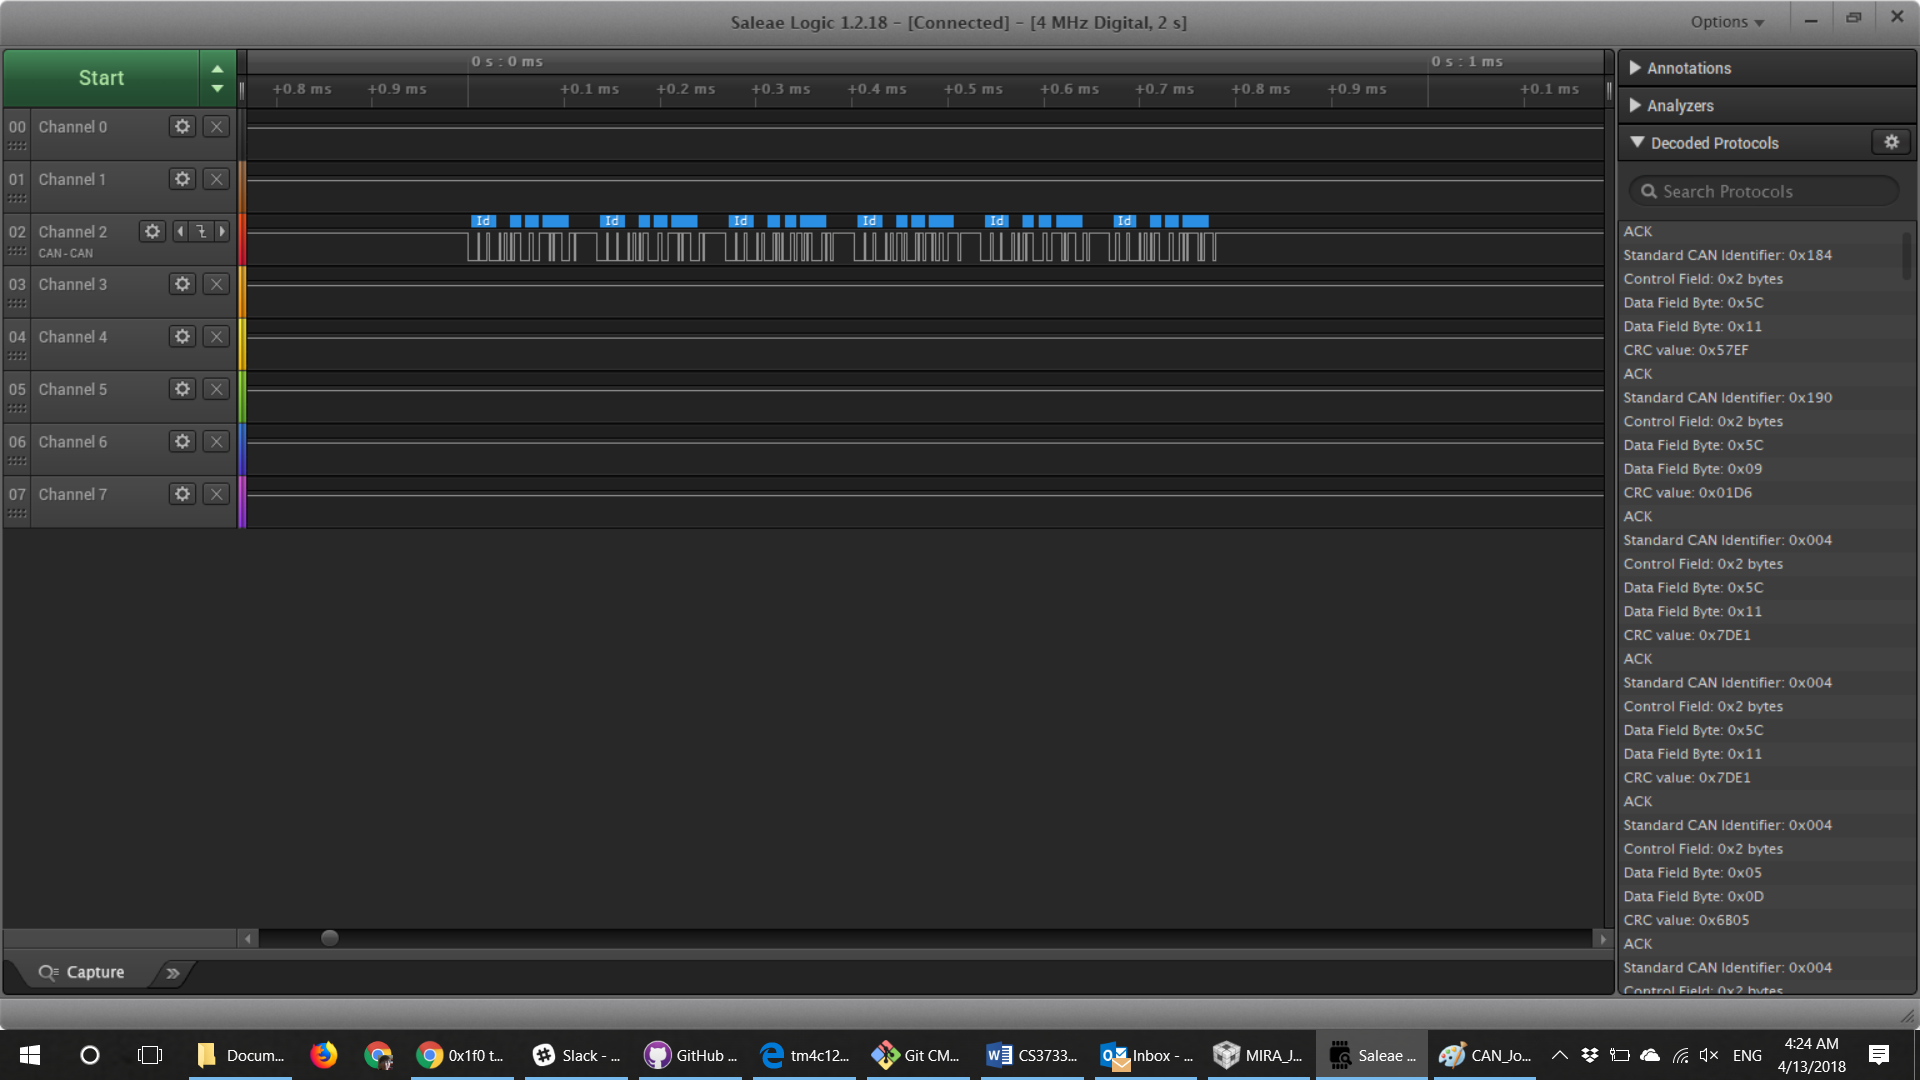
\includegraphics[width=\textwidth]{CAN_Joint_Update}
	\caption{Position update from the base module}
	\label{fig:can_joint_update}
\end{figure}

\begin{figure}[H]
	\centering
	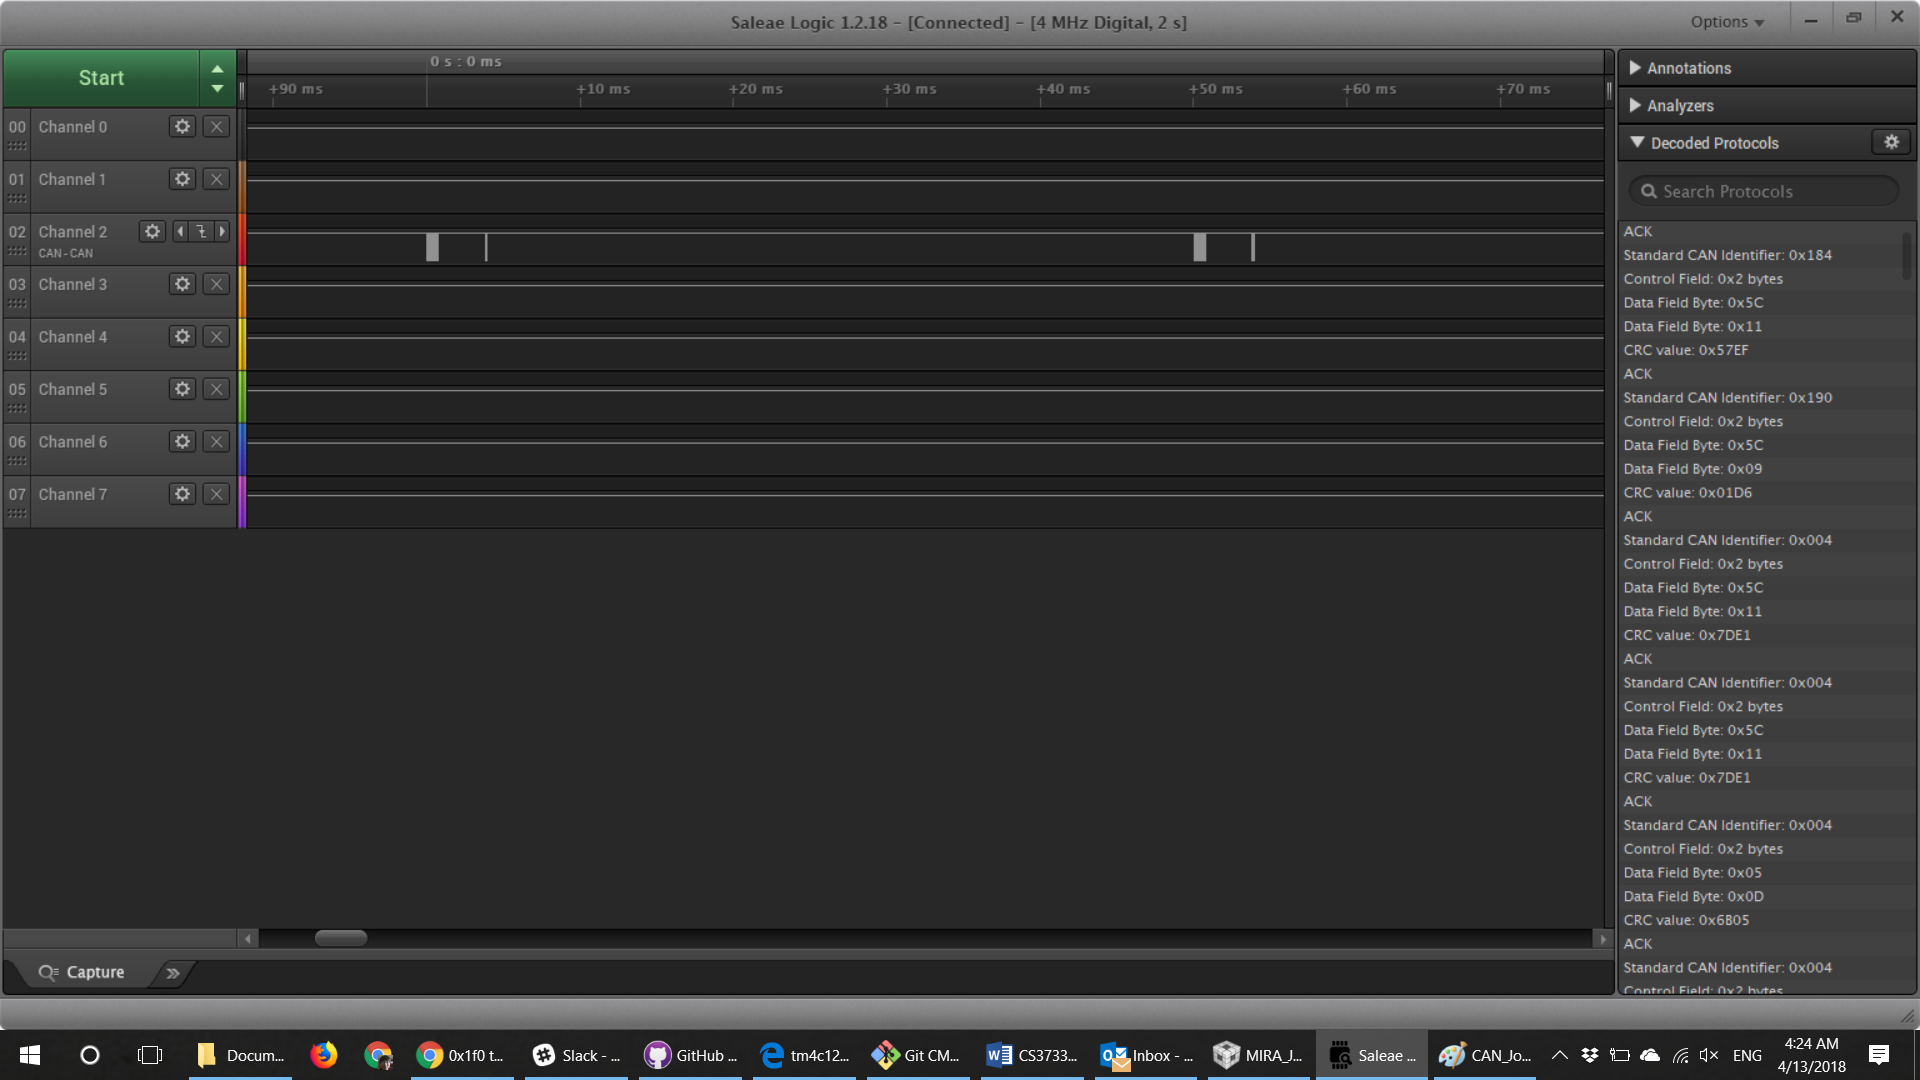
\includegraphics[width=\textwidth]{CAN_Joint_Update_response}
	\caption{Position update from the base module with response from a joint}
	\label{fig:can_joint_update_response}
\end{figure}

\subsection{Base Module}
The base module serves two main purposes. The first is to translate serial UART packets from the computer to the CAN packets for the joints. The second is to provide power and communication buses for the entire system. These two parts are crucial to the functionality of the arm.

\subsubsection{Overview of Base Module Design}
The base module is pretty simple from a hardware standpoint. It mostly consists of two parts, the microcontroller and the power supply. A CAN transceiver is needed, in addition to the microcontroller, but after that there is no more hardware except connectors. A block diagram can be seen in Figure \ref{fig:base_block_diagram}.

\begin{figure}[H]
	\centering
	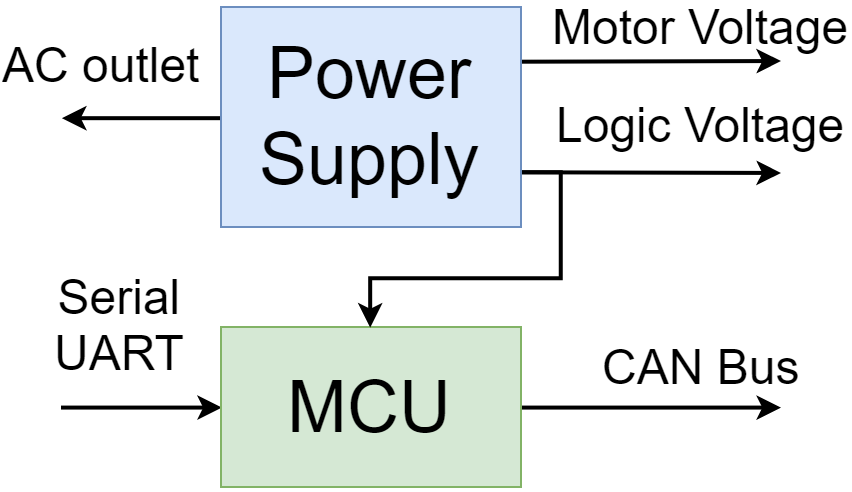
\includegraphics[scale=0.3]{base_block_diagram}
	\caption{Block diagram of the base module}
	\label{fig:base_block_diagram}
\end{figure}

\subsubsection{Base Module Code}
The base module is also running TI RTOS for TivaWare boards. The main reason for this was to multithread the code to simplify programming. By having multiple threads, the code can be compartmentalized into sections that handle different parts. Figure \ref{fig:base_code_flowchart} shows the code flowchart. There are two main states, initialization and runtime. During initialization, all of the constants for each joint are loaded in. These include CAN ID, encoder offset, and PID constants. Once all 6 joints have been initialized, the code transmits that information on the CAN bus and switches into the runtime state. 

\noindent In the runtime state, the base module reads in joint angle updates from the computer, then sends them along to the corresponding joint. The joints then send back their actual joint angle, which is parsed back into serial and sent to the computer. The code repository containing all of this code can be found in Appendix \ref{app:code_repo}.

\begin{figure}[H]
	\centering
	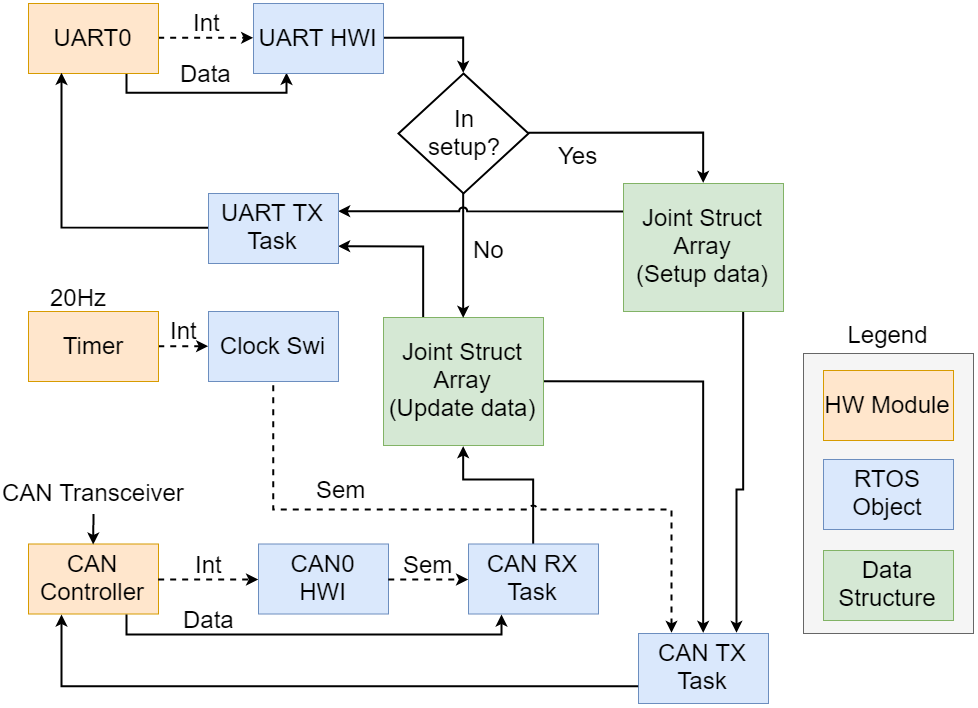
\includegraphics[scale=0.4]{base_code_flowchart}
	\caption{Base module code flowchart}
	\label{fig:base_code_flowchart}
\end{figure}

\subsubsection{Power Rails}
Since the arm is of a variable size, the power rail must also be modular enough to accomodate this. To solve this issue, a modular power rail was designed, and a diagram can be seen in Figure \ref{fig:power_rail}. The main rail is made up of 16 AWG wire and the connectors are rated for 15A continuous current draw. The power rail and CAN bus are very similar, but with smaller amperage JST connectors and thinner, 22 AWG wire.

\begin{figure}[H]
	\centering
	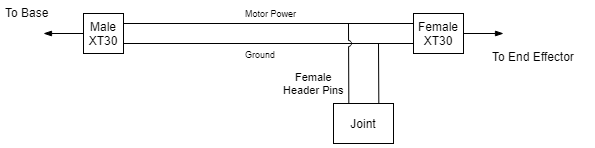
\includegraphics[width=\textwidth]{ModularPower}
	\caption{Modular power rail for motor power}
	\label{fig:power_rail}
\end{figure}

\subsection{Arm Structure}
Arm structure is not something we wanted to fully define, since the end user is supposed to create their own arms, but there were some basic components that needed clarification. The first of these is that every arm must begin with a base module and have some combination of up to five additional joints connected.  This allows the end-user flexibility in how they want to construct the arm without allowing them to add too many joints. 


\subsection{Software Application}
The code library is another important part of what we did to make our arm work. It controls all of the electrical components via the sending of packets out to the base module over a Serial UART line. It handle a lot of the more involved calculations for controlling the arm like the forward and inverse kinematics. The repository containing all of the software code can be found in Appendix \ref{app:code_repo}.


\subsubsection{Maven}
Maven is a utility for Java-based projects that seeks to provide a uniform build system for the project. It accomplishes this by defining a project object model and a set of plugins that each Maven project shares. Therefore, Maven can provide a streamlined build environment for every instance of the project, allowing users to have the same build process across multiple different devices and environments. Maven could be compared to a flexible template for how a project should be arranged and what files should be included. We chose Maven for our Java project because it makes it much easier for our team to collaborate on the front-end side of the code.  It also allows us to package into our program libraries that we used in our project so that there are fewer dependencies that the end-user must download in order to use our software \cite{maven}.


\subsubsection{Program flow}

\begin{figure}[H]
\centering
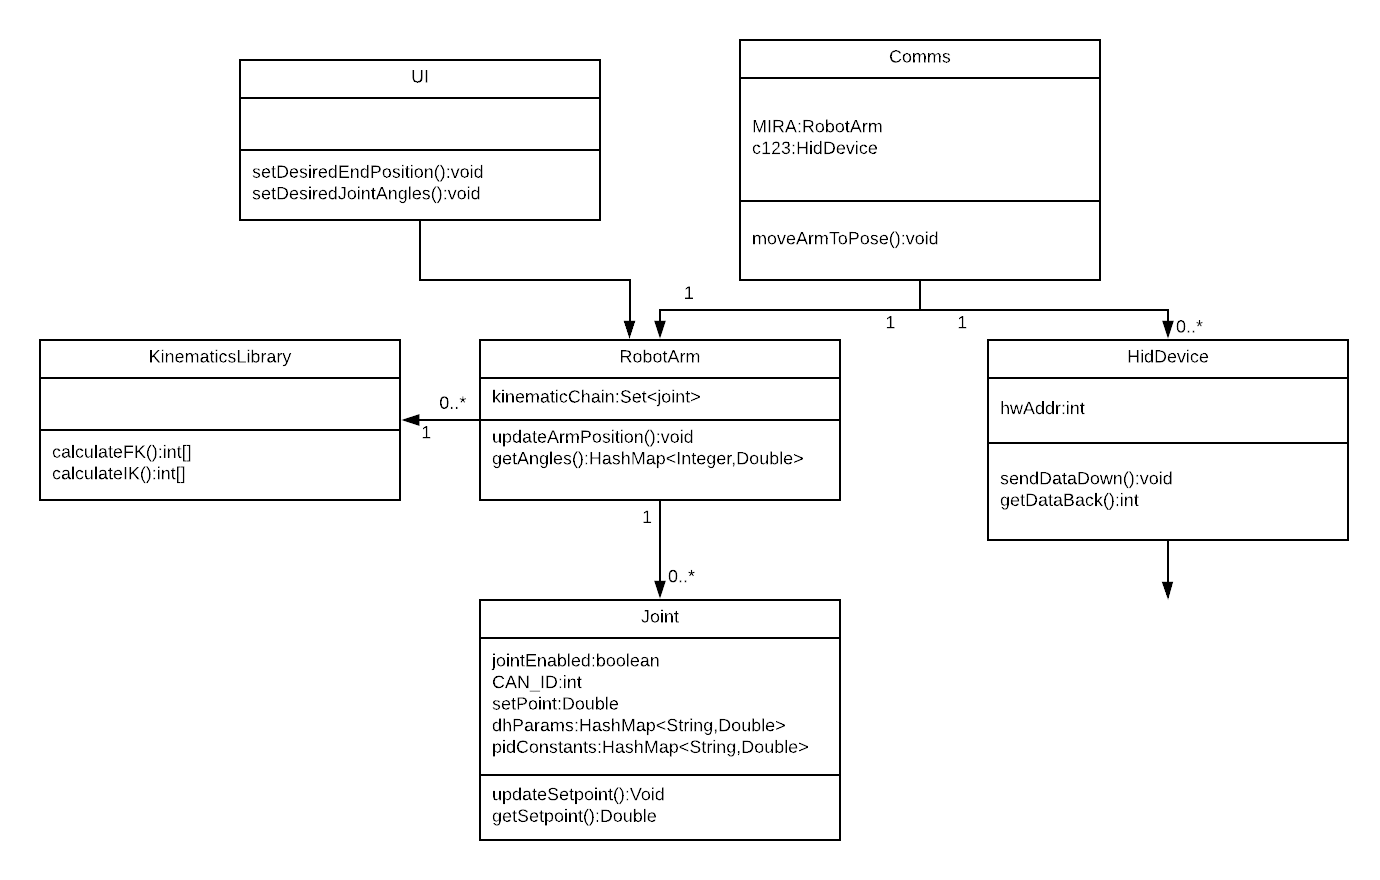
\includegraphics[width=\textwidth]{pc_Mira_UML}
\caption{UML Diagram showing different classes and their relations}
\label{fig:Functional_Block_Diagram}
\end{figure}

%TODO do something more with this sentence
\noindent The front-end program running on the PC is written in Java. We used JavaFX to make the GUI. We chose to write this part of the program in Java because of the speed and reliability of a language that has many libraries and excellent Interactive Development Environments.  

\noindent The main class starts the JavaFX Project. The JavaFX Project holds an list of joints which lists all the joints, which contains data about how the arm is configured. Each Joint object makes sure to tell the Comms object that it's time to send a message to the actual joint whenever new information about itself comes in. When the user enters new information about the arm into the GUI, the GUI's controller tells the joint object to change that information about itself. For example, if the user changes the setpoint of Joint 2 from 90 degrees to 112 degrees, the GUI will tell Joint 2 that its position has been updated to 112. Joint 2 will, upon seeing that its position has been updated, ask the Comms object to convey the new position information to the arm's base board.

\noindent The Joint object does not contain a Comms object inside itself. Rather, there is a single Comms object for the entire program to use. The Comms object follows the Singleton design pattern. A singleton is a class which can only ever be instantiated one time. Singletons are often used to hold configuration information about a program because they guarantee that if one object makes changes to the singleton's settings then any other object that subsequently asks for those settings will get back the most up-to-date version.

\noindent In this case, it makes sense to use a singleton because we want to guarantee that there's only a single place in the code which tries to access the serial port at any given time. Another way to accomplish this same goal would have been to move all of Comms's functions to inside the JavaFX controller. There is only one controller object. Arranging the program this way would have violated Java's design principles and would have made writing the code a battle rather than an art form. %Please don't take this out they're definitely not going to get this far into the paper anyway probably

\noindent Each joint would need to hold a reference to the JavaFX controller inside itself. Referencing such an architecture-specific piece of the program within the core of the program's logic would be bad for future portability of the code. 

\subsubsection{Serial Communication}
Serial communication is a very common protocol used to transmit data between a maximum of two devices over two lines, Rx and Tx. Serial communication is already available on our microcontroller through its universal asynchronous receiver/transmitter (UART). This device translates the Tx and Rx line into a parallel data bus that can interface with our microcontroller autonomously. The Java code interfaces directly with this UART over a USB line connected to both the Tiva board and the computer. The Java code holds a class called Comms which opens a specified serial port upon instantiation. This is implemented through the use of NRJavaSerial \cite{NRJavaSerial}, a library created by Kevin Harrington used for serial communications over USB. Upon instantiation of the Comms singleton, we open the specified serial port on the computer and begin polling it at a baud rate of 115200 bits/second. The enables the port to send and receive data so that the computer can send and receive packets from our base board. The Java code holds a buffer which acts as a First in First Out (FIFO) queue that is constantly updated when new data is received so that we can read in data that is on the serial line \cite{SerialSparkfun}.
Since we are only able to send individual bits at a time across the serial line, we need to encode and decode the data that we send.  We have to encode the data from ASCII strings into their decimal equivalents before sending them out over the serial line. Then upon receipt of data we must decode the data before it is able to be built into a string which represents one packet. Once we have individual packets available to us as strings, we can easily use Java's string comprehension functionality to update the necessary parts of the code and properly encode data for sending\cite{SerialSparkfun}.

\subsubsection{Mutltithreading}
Multithreading is the process of creating new threads in order to run code in parallel. Creating a new thread in Java involves instantiating a new thread object from Java's standard libraries and passing in the relevant information to the Thread through the constructor \cite{ThreadJava}. The reason that we needed to use a thread is the need for a mode where the computer communicates over Serial, writing out and reading in data that it receives at a constant rate. The problem with this style of coding is that it requires a while loop which continuously executes code that would normally block all other pieces of code from running. Since we need to concurrently run our GUI and modify the values that we are sending to the arm based on GUI inputs, we cannot have the processor locked up all the time sending and receiving serial communications. Therefore, we created a new thread where serial communications could be handled on an entirely separate process than the GUI. We create this thread after the initialization of our arm has been completed and start it when the arm has acknowledged that it is ready to begin communications. Therefore, we are able to uphold constant serial communications without causing our GUI to crash mid-operation. Doing this allows us to move the joint sliders pictured below and have them constantly send out new messages to the arm telling the selected joint to turn to the new position. 

\begin{figure}[H]
	\centering
	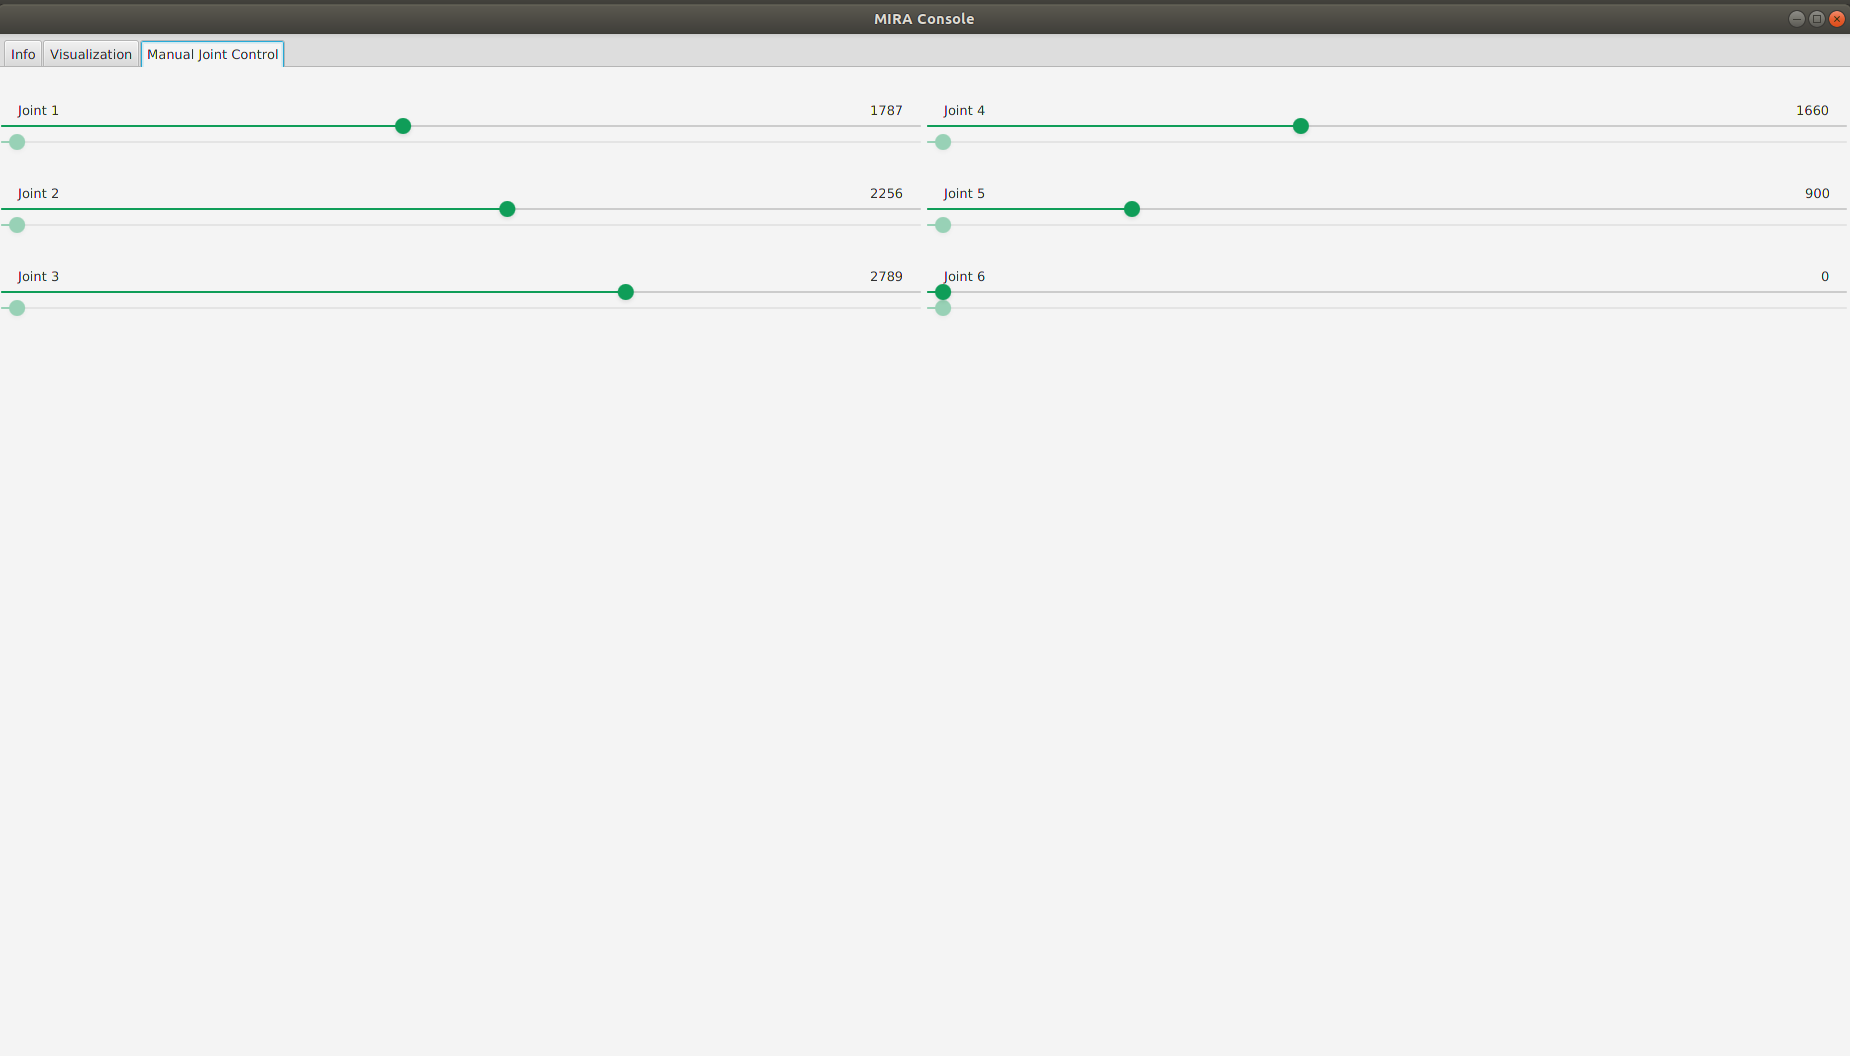
\includegraphics[width=\textwidth]{GUI_sliders}
	\caption{Image of the GUI tab which adjusts the setpoint for joints}
	\label{fig:GUI_Sliders}
\end{figure}


\subsubsection{Saving of Configuration}
In order to store the information that we need to be persistent between different instances of the application, we used a library called Gson made by Google \cite{gson}. This library's primary use is to take data and store it in a .json file, a kind of simplistic database.  We used this library to save the joint object which were the data containers about the configuration of the arm. All of the saving and loading is done via the GUI so that the user can either load information about an arm themselves, or they can change the values using the GUI text fields and save a new configuration when it needs updating. Doing so allows the user to always be able to either modify and update the constants inside the data container that is the Joint object and have those objects be saved and loaded during each runtime of the application. Pictured below is the GUI tab which stores all of the constants for the arm such as encoder home values and PID constants, as well as has buttons to interface with the saving, loading and startup of our program.

\begin{figure}[H]
	\centering
	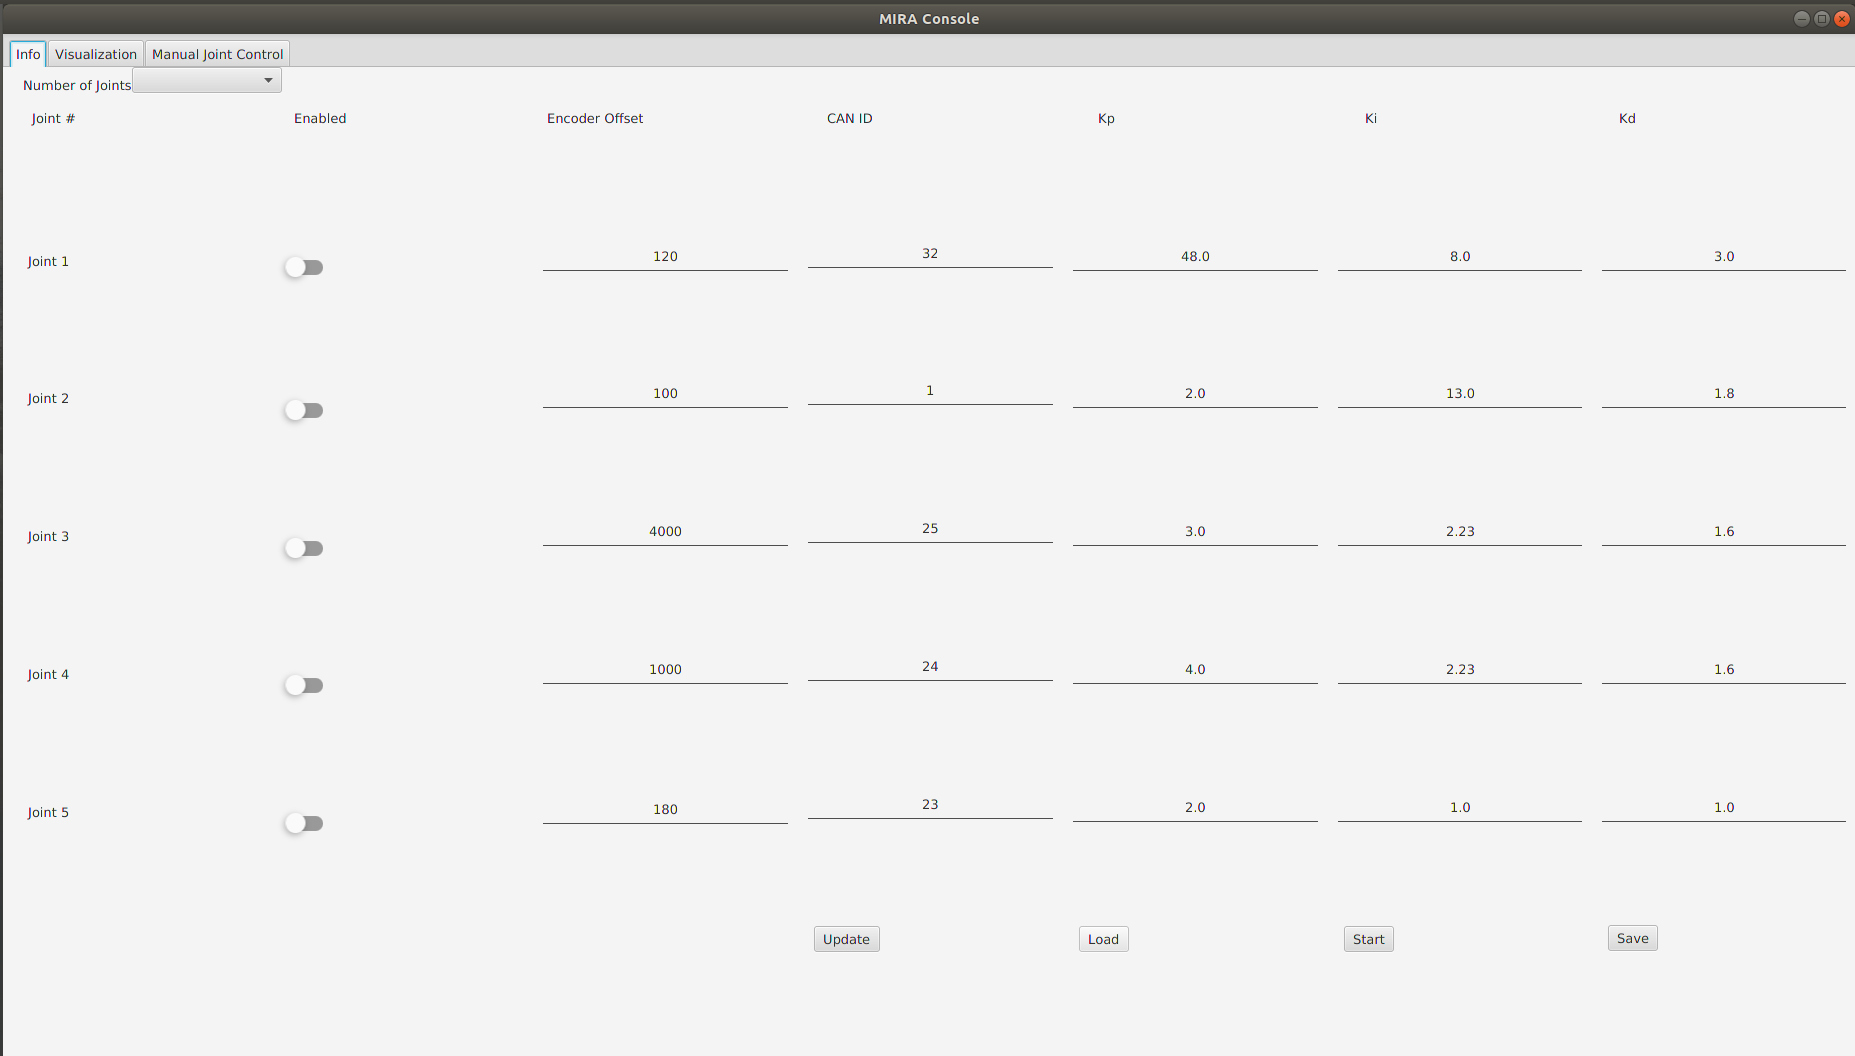
\includegraphics[width=\textwidth]{GUI_config}
	\caption{GUI config tab with save and loading}
	\label{fig:GUI_config}
\end{figure}






